% =====================================================================
%  Geometric Algebra Lifts and Scalar Floquet Criteria for Switched Power Converters
%  Manuscript source, IEEE Transactions on Circuits and Systems I
% =====================================================================
\documentclass[journal]{IEEEtran}
\input{glyphtounicode}
\pdfgentounicode=1
\usepackage{amsmath,amssymb,amsthm}
\usepackage{bm}
\usepackage{graphicx}
\usepackage{booktabs}
\usepackage{array}
\usepackage{multirow}
\usepackage{cite}
\linespread{0.92}

% ---------------------------------------------------------------------
%  Marcado de lo anadido tras la campana de validacion.
%  Para imprimir en negro: cambiar \nuevotrue por \nuevofalse. Nada mas.
% ---------------------------------------------------------------------
\usepackage{xcolor}
\newif\ifnuevo
\nuevofalse
\newcommand{\nuevo}[1]{\ifnuevo\textcolor{blue}{#1}\else#1\fi}

\newtheorem{proposition}{Proposition}
\newtheorem{definition}{Definition}
\newtheorem{lemma}{Lemma}
\newtheorem{corollary}{Corollary}
\newcommand{\Gnn}{\mathcal{G}(n,n)}
\newcommand{\rev}[1]{\widetilde{#1}}
\newcommand{\sgn}{\operatorname{sign}}

\begin{document}

\title{Geometric Algebra Lifts and Scalar Floquet Criteria\\
for Switched Power Converters}

\author{Francisco~G.~Montoya and~Alfredo~Alcayde%
\thanks{The authors are with the Department of Engineering, University of
Almer\'ia, 04120 Almer\'ia, Spain (e-mail: pagilm@ual.es).}}

\maketitle

\begin{abstract}
The stability of a periodic orbit of a switched converter is governed
by its monodromy matrix, a product of transition and saltation
matrices. We show that this product lifts to the geometric algebra
$\Gnn$: every nonsingular factor becomes a versor and the
monodromy a single geometric product. The saltation of an event
lifts to the element $1+\bm{u}\bm{n}$ built from its field jump and
surface normal; one scalar, the sign of $\det S_k$, classifies
the event as pass-through, reflection-type or singular, and the rapidity
$\ln\lvert\det S_k\rvert$ places continuous and discontinuous conduction and
the deadbeat ramp slope on two hyperbolic sheets. The spinor norm of
the versor gives the sign of $\det M$ as the parity of the number of
reflection-type events, so an odd count forces
a real negative Floquet multiplier; its scalar and pseudoscalar parts are
proportional to $\det(I+M)$ and $\det(I-M)$, so a flip or a fold boundary is
the zero of one scalar and, for second-order converters, three scalars of the
unnormalized lift form a complete stability test. For an even count in a
two-phase converter, the interference between the two reflections decides
between a torus and a period doubling, with the mismatch threshold in closed
form. Simulations of lossy buck, boost and interleaved
converters and published multipliers of the voltage-mode buck converter
confirm the predictions and give the gap to the classical ramp rule in closed
form.
\end{abstract}

\begin{IEEEkeywords}
Border collision, DC--DC converters, discontinuous conduction mode, Floquet
theory, geometric algebra, interleaved converters, saltation matrix,
subharmonic oscillation.
\end{IEEEkeywords}

\begin{table}[!t]
\caption{Nomenclature}
\label{tab:nomen}
\centering
\footnotesize
\setlength{\tabcolsep}{4pt}
\begin{tabular}{@{}ll@{}}
\toprule
\multicolumn{2}{@{}l}{\emph{Circuit and Floquet quantities}}\\
$\bm{x}$, $\delta\bm{x}$ & state vector; perturbation about the orbit \\
$T$, $D$ & switching period; duty cycle \\
$A_j$, $\bm{b}_j$ & state matrix and input of topology $j$ \\
$\Phi_i$, $\tau_i$ & state-transition matrix and duration of interval $i$ \\
$h_k$, $\dot h_k^{\mp}$ & switching function of event $k$; its crossing
                          velocities \\
$\bm{f}_k^{\mp}$ & vector fields before and after event $k$ \\
$\bm{u}_k$ & normalized field jump at event $k$, \eqref{eq:saltation} \\
$\bm{n}_k$ & covector $\nabla_{\bm{x}}h_k$ normal to the surface \\
$S_k$, $F_k$ & saltation matrix $I+\bm{u}_k\bm{n}_k^{T}$; rank-one factor \\
$M$, $\mu$ & monodromy matrix; Floquet multiplier \\
$m_1$, $m_2$ & rising and falling inductor-current slopes \\
$m_a$, $I_{\mathrm{ref}}$ & compensation-ramp slope; current reference \\
\addlinespace[2pt]
\multicolumn{2}{@{}l}{\emph{Scalars carrying the geometry}}\\
$\sigma_k$ & $\bm{n}_k^{T}\bm{u}_k$, so that $\det S_k=1+\sigma_k$ \\
$\lambda_k$ & rapidity, $\ln\lvert1+\sigma_k\rvert$ \\
$N_r$ & negative-determinant factors per period ($\det F_k<0$) \\
$\Delta\mu$, $\chi$ & mismatch and interference of two reflections, \eqref{eq:par} \\
\addlinespace[2pt]
\multicolumn{2}{@{}l}{\emph{Geometric algebra} (boldface)}\\
$\Gnn$ & geometric algebra of neutral signature \\
$\bm{e}^{\pm}_i$ & orthonormal basis,
                   $(\bm{e}^{\pm}_i)^2=\pm1$ \\
$\bm{w}_i$, $V_w$ & null basis and subspace of vectors ($\bm{x}$, $\bm{u}_k$) \\
$\bm{v}_i$, $V_v$ & dual null basis and subspace of covectors ($\bm{n}_k$), \\
           & with $\bm{w}_i\!\cdot\!\bm{v}_j=\tfrac12\delta_{ij}$ \\
$\bm{B}_k$, $\hat{\bm{B}}_k$ & saltation plane $2\,\bm{u}_k\wedge\bm{n}_k$;
                               its normalization \\
$\bm{Q}_M$ & lift of $M$, with $\bm{Q}_M\rev{\bm{Q}}_M=\det M$ \\
$\bm{W}$, $\rev{\bm{W}}$ & normalized lift, $\bm{W}\rev{\bm{W}}=\sgn\det M$; reverse \\
$\langle\cdot\rangle_0$ & scalar part, $2^n\langle\bm{Q}_M\rangle_0=\det(I+M)$ \\
$\bm{\Gamma}$ & $\prod_i\bm{e}^{+}_i\bm{e}^{-}_i$, $2^n\langle\bm{Q}_M\bm{\Gamma}\rangle_0=\det(I-M)$ \\
\bottomrule
\end{tabular}
\end{table}

\section{Introduction}
\IEEEPARstart{S}{witched} power converters operate on periodic orbits rather
than on equilibria, and averaged models cannot see the fast-scale
instabilities that develop at the switching frequency
\cite{deane1990instability,banerjee2001nonlinear}. Floquet theory captures
them. A small perturbation of the orbit is propagated over one switching
period by the monodromy matrix $M$, and the orbit is asymptotically stable
when every Floquet multiplier, every eigenvalue of $M$, lies inside the unit
circle. A real negative multiplier reverses the sign of its perturbation from
one cycle to the next; the perturbation decays while $\lvert\mu\rvert<1$, and
the period-doubling boundary is reached at $\mu=-1$. For piecewise-linear
converters, $M$ is the product of the matrix exponentials of the intervals and
of the saltation matrices, the first-order corrections at the instants where
the state itself triggers a switching
\cite{aizerman1958,muller1995,leine2004,kong2024saltation}. Since the
saltation-based stability analysis of the buck converter in this journal
\cite{giaouris2008stability}, the monodromy approach has become standard
\cite{elaroudi2015review}. It explains subharmonic oscillation in
current-programmed converters \cite{elaroudi2021analytical}, the classical
compensation-ramp rule \cite{deane1990instability,erickson2020fundamentals}
and its nonlinear variants \cite{elaroudi2020piecewise}, it extends to
resonant converters with many switching events per period
\cite{mandal2013symmetry} and to interleaved topologies
\cite{wu2014interleaved}, and it underlies the Filippov-based treatment of
subharmonic instability \cite{giaouris2009filippov}. We use saltation matrices in the hybrid-system
sense, as the linearization across a state-triggered event with its own reset
logic, and not only for transversal crossings of a Filippov discontinuity
surface. Section~\ref{sec:prelim} shows why the distinction matters: the
class of events on which our parity rule rests cannot occur at a transversal
crossing.

This paper rewrites the construction in the language of geometric algebra.
The factors of the monodromy have geometric content, contraction by the
flows and a rank-one update at each switching, and the algebra represents
each factor by an object whose scalar invariants can be read before the
product is formed. Our starting point is a result of Doran, Hestenes, Sommen
and Van Acker \cite{doran1993lie}: the identity component
$GL^{+}(n,\mathbb{R})$ of the general linear group is represented by rotors
of the algebra $\Gnn$ of neutral signature acting on a null subspace. We lift
the converter state to that subspace. Every nonsingular factor of the
monodromy, interval flow or saltation, becomes a versor, and $M$ becomes a
single geometric product. The orientation-reversing factors that latched
switching creates require the elements with $\bm{W}\rev{\bm{W}}=-1$, which
\cite{doran1993lie} excludes by construction and the Clifford--Lipschitz
group readmits \cite{lounesto2001}. The representation is exact. It involves
no averaging and no commutation assumption between topologies, and it
accommodates conduction losses and parasitics.

Five results follow. First, the saltation of event $k$ lifts to the single
element $1+\bm{u}_k\bm{n}_k$ of $\Gnn$, whose spinor norm is $\det S_k$
(Proposition~\ref{prop:species}). The sign of that scalar classifies the
event as pass-through, as reflection-type when the switching reverses the
velocity of the switching function, or as singular when it annihilates that
velocity, in which case the saltation is a projector and no versor exists.
The type belongs to the operating point, not to the detector. In
peak-current control the three types are separated by the compensation-ramp
slope, and the singular boundary is the classical deadbeat slope. Second, the
rapidity $\lambda=\ln\lvert\det S_k\rvert$ places the operating regimes of a
converter on a pair of hyperbolic sheets joined at
the singular value, with
discontinuous conduction at the end $\lambda=-\infty$
(Section~\ref{sec:invariants}). Third, a parity rule
(Proposition~\ref{prop:parity}). Let $N_r$ be the number of reflection-type
events per period. If every event is nonsingular, transversal and separated,
the spinor norm of the total versor is
$\bm{W}\rev{\bm{W}}=(-1)^{N_r}=\sgn(\det M)$. At the matrix level this is the
multiplicativity of the determinant. Its content is that latched,
reflection-type switchings are the only source of orientation reversal in a
converter cycle: a smooth
flow has $\det M=\exp(\int\operatorname{tr}A\,dt)>0$ by Liouville's formula, so no arrangement of smooth intervals can force a
real negative multiplier, and an odd count of reflections does. For a
second-order converter an odd count also forces the whole spectrum to be
real. Fourth, the lift carries the characteristic polynomial
(Proposition~\ref{prop:grades}). The scalar and pseudoscalar parts of the
unnormalized lift are $\det(I+M)$ and $\det(I-M)$, so the flip boundary is
the zero of one scalar and the fold boundary the zero of another; for
second-order converters the three scalars $\bm{Q}_M\rev{\bm{Q}}_M$,
$\langle\bm{Q}_M\rangle_0$ and $\langle\bm{Q}_M\bm{\Gamma}\rangle_0$ form a
complete stability test, with no eigenvalue computed. Fifth, the even case of
the parity rule is decided for two-phase converters
(Section~\ref{sec:par}). Two reflection-type events that interact through the
output capacitor produce a complex pair near $-1$ when the corresponding
determinants differ by less than a threshold obtained in closed form. The
orbit then loses stability through a Neimark--Sacker bifurcation with a slow
modulation of the subharmonic, and otherwise through a period doubling.

Several of these statements have classical matrix counterparts. The
determinant of a rank-one update, the multiplicativity of the determinant and
the Schur--Cohn conditions are standard, and the zeros of $\det(I\pm M)$ are
the usual test functions for flip and fold bifurcations in numerical
continuation \cite{kuznetsov2004}. Moreover, by
Proposition~\ref{prop:grades} every scalar of the lift is a polynomial in the
entries of $M$, and no number obtained here is out of the reach of matrix
methods. Table~\ref{tab:aporta} separates the classical content of each
result from the contribution of this paper, which is of two kinds. The first
consists of statements about converters that hold in either language and, to
our knowledge, have not been reported: 1) a reflection-type event
requires a latch and cannot occur at a Filippov crossing; 2) the deadbeat
ramp slope is the boundary between event types; 3) a delayed sampler is a
rank-one factor with negative determinant for every positive gain; 4) the
corrected saltation matrix of hybrid differential-algebraic models follows
from the covector reading; 5) at a coupled simultaneous corner the
reflection count depends on the event order; and 6) in a two-phase converter
the mismatch between the two reflections, compared with the interference
between them, decides between a torus and a period doubling. The second is
structural. The
lift is multiplicative in the factors of the cycle and, at the same time, the
characteristic polynomial is read from it linearly. With matrices, $M$ has
the first property only, whereas the compound matrices of $M$ have both, and
the lift is their direct sum (Section~\ref{sec:grades}).

\begin{table}[!t]
\caption{Classical Content and Contribution of Each Result}
\label{tab:aporta}
\centering
\footnotesize
\setlength{\tabcolsep}{3pt}
\begin{tabular}{@{}>{\raggedright\arraybackslash}p{0.15\columnwidth}>{\raggedright\arraybackslash}p{0.37\columnwidth}>{\raggedright\arraybackslash}p{0.42\columnwidth}@{}}
\toprule
Result & Classical matrix fact & Contributed here \\
\midrule
Prop.~\ref{prop:species} & $\det(I+\bm{u}\bm{n}^{T})=1+\bm{n}^{T}\bm{u}$; zero
multiplier of a singular saltation \cite{muller1995,kong2024saltation} &
event types from the sign of $\dot h^{+}/\dot h^{-}$; a latch is required for
reflection; one element $1+\bm{u}\bm{n}$ for all types \\
\addlinespace[2pt]
Eq.~\eqref{eq:budget} & Liouville's formula; multiplicative determinant &
rapidity of each event; closed-form gap to the ramp rule, \eqref{eq:gap} \\
\addlinespace[2pt]
Prop.~\ref{prop:parity} & multiplicative determinant & sign of $\det M$ from
a count of circuit events; dependence on the operating point and on the model \\
\addlinespace[2pt]
Sec.~\ref{sec:par} & torus of a two-phase boost converter; period doubling
suppressed by symmetry & criterion $\lvert\Delta\mu\rvert<2\chi$;
interference and modulation frequency in closed form \\
\addlinespace[2pt]
Prop.~\ref{prop:grades} & $\operatorname{tr}\Lambda^{k}M$
\cite{horn2013matrix}; test functions $\det(I\pm M)$ \cite{kuznetsov2004};
Schur--Cohn test & characteristic polynomial as linear functionals of one
multiplicative object \\
\addlinespace[2pt]
Secs.~\ref{sec:retardo}, \ref{sec:esquina} & --- & sampler as a rank-one
factor; order-dependent count at coupled corners \\
\bottomrule
\end{tabular}
\end{table}

Three lines of work are related. Geometric algebra has an established record
in power theory \cite{montoya_gapot1,montoya_gapot3} and in
three-phase system control \cite{velasco2025introducing}.
Sira-Ram\'irez and coworkers have applied it to Lyapunov stability of smooth
systems \cite{sira2022lyapunov} and to sliding-mode and invariance control of
switched systems \cite{sira2023sliding,sira2023invariance,sira2025hamiltonian},
that is, to the averaged dynamics on a switching manifold at ideally infinite
switching frequency; Derevianko and Va\v{s}\'ik address switching-path
synthesis \cite{derevianko2024solverfree}. We treat the complementary
problem, the cycle-to-cycle map at finite fixed frequency and the stability of
the period-one orbit. The border-collision literature classifies
piecewise-linear maps by orientation, that is, by the sign of the determinant
on each side of the border
\cite{ghosh2025robust,simpson2025zero,fatoyinbo2023synopsis}, and the
CCM--DCM transition was identified early as a border collision with a change
of state-space dimension \cite{parui2002border}. Ghosh, McLachlan and Simpson
trace the orientation reversal of a boost converter to the latched switching
that is called reflection here \cite{ghosh2025robust}. In those studies the
signs are parameters of a map that has already been extracted; the
correspondence with the present results is stated in
Section~\ref{sec:sheets}. Finally, for symmetric two-phase operation the
even-parity case agrees with the suppression of period doubling in symmetric
systems \cite{swift1984suppression}, as discussed in
Section~\ref{sec:invariants}.

Every claim is verified in simulation on converter models with conduction
losses, capacitor ESR, diode forward drop and component tolerances
(Section~\ref{sec:validation}). The exact subharmonic boundary separates
measurably from the classical ramp rule once losses are included, and the
volume budget gives the gap in closed form. An independent event-driven
simulation identifies a monodromy that matches the versor prediction to
better than $10^{-4}$ in every multiplier, determinant sign included. The
parity rule holds on two- and three-phase interleaved converters with
mismatched components, and one sweep of the current reference displays the
rapidity sheets from DCM to duty saturation. We then read the rule against
Floquet data published by others for topologies we did not build, including
a photovoltaic model with an algebraic constraint whose corrected saltation
matrix \cite{hayes2020application} the covector formulation reproduces
(Section~\ref{sec:campana}). A voltage-mode buck converter and a boost
converter extend the tests to a different switching logic and a different
topology, and the former is compared with published multipliers and
experimental waveforms \cite{giaouris2008stability}
(Section~\ref{sec:otros}). No hardware was built for this paper. Scripts that
reproduce every figure and table accompany the paper as supplementary
material. Section~\ref{sec:prelim} follows one switching period of a buck
converter and defines the saltation matrix, Section~\ref{sec:versors} lifts
the construction to $\Gnn$, Section~\ref{sec:invariants} derives the scalar
invariants, Section~\ref{sec:validation} tests them, and
Section~\ref{sec:discussion} states what a designer gains.

\section{Preliminaries: Floquet Analysis of Switched Converters}
\label{sec:prelim}
Fig.~\ref{fig:tutorial} shows one period of a buck converter under
peak-current control, the simplest of the platforms used in
Section~\ref{sec:validation}; Table~\ref{tab:nomen} collects the notation.
The state $\bm{x}=(i_L,v_C)$ consists of the inductor current and the
capacitor voltage. A clock closes the switch at the start of every period
$T$. The current rises at rate $m_1$ until it reaches the reference
$I_{\mathrm{ref}}-m_at$, where $m_a$ is the slope of the compensation ramp;
the comparator then opens the switch, and a latch holds it open until the
next clock edge while the current falls at rate $m_2$. The fraction $D$ of
the period with the switch closed is the duty cycle. The ramp is the
classical remedy for the subharmonic oscillation of this control, in which
the orbit of period $T$ gives way to one of period $2T$.

A perturbation of the state at the start of the period changes the instant at
which the current reaches the reference (Fig.~\ref{fig:tutorial}(b)). The
continuous state is not reset at the switching, but the two trajectories,
compared at the same time, differ by more than the smooth intervals account
for, because the switch opened earlier or later than it should. The
saltation matrix is this correction to first order. The monodromy matrix
combines it with the propagation through the two switch configurations and
maps the perturbation at the start of one period to the perturbation at the
start of the next. Fig.~\ref{fig:tutorial}(c) shows the switching function
$h=i_L-(I_{\mathrm{ref}}-m_at)$ along the period. With a shallow ramp it
touches zero and returns to the side it came from; with a steep ramp it
crosses. That difference decides the sign of the saltation determinant, and
it runs through the whole paper.

\begin{figure}[!t]
\centering
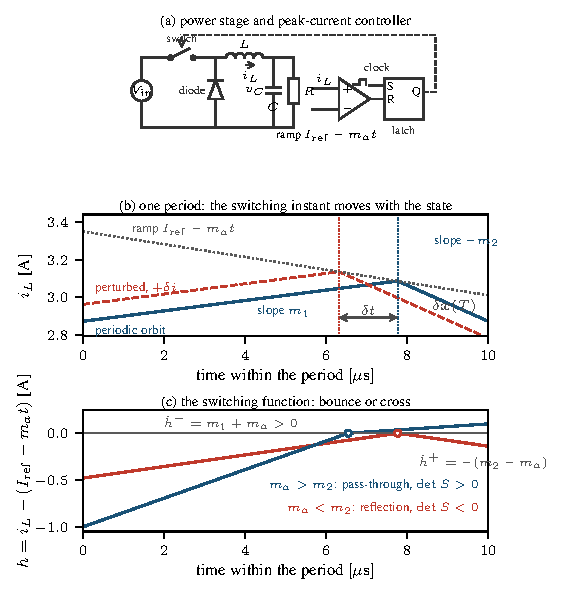
\includegraphics[width=\columnwidth]{figs/tutorial_saltacion.pdf}
\caption{One period of the peak-current-controlled buck of
Section~\ref{sec:ramp}. (a)~Power stage and controller. The clock sets the
latch and closes the switch; the comparator resets it when $i_L$ reaches the
ramp $I_{\mathrm{ref}}-m_at$. (b)~Inductor current of the periodic orbit
(solid) and of a trajectory started $\delta i$ higher (dashed). The perturbed
current reaches the ramp earlier by $\delta t$, and the two trajectories
differ at the end of the period by the vector $\delta\bm{x}(T)$ that the
monodromy predicts to first order. (c)~Switching function
$h=i_L-(I_{\mathrm{ref}}-m_at)$ for two ramp slopes, with velocities
$\dot h^{-}=m_1+m_a$ before the event and $\dot h^{+}=-(m_2-m_a)$ after it.
For $m_a<m_2$ the function touches zero and returns, a reflection-type event
with $\det S<0$; for $m_a>m_2$ it crosses, a pass-through event with
$\det S>0$.}
\label{fig:tutorial}
\end{figure}

For a general converter, let the state $\bm{x}\in\mathbb{R}^n$ satisfy
$\dot{\bm{x}}=A_j\bm{x}+\bm{b}_j$ in switch configuration $j$, with
transitions either at clock edges or at state-triggered events
$h_k(\bm{x},t)=0$. Let the periodic orbit have period $T$ and state-triggered
events at the instants $t_k$. Linearized about the orbit, a perturbation
propagates over one period as $\delta\bm{x}(T)=M\,\delta\bm{x}(0)$ with
\begin{equation}
M=\Phi_{m}\,S_{K}\,\Phi_{m-1}\cdots S_{1}\,\Phi_{0},\qquad
\Phi_i=e^{A_{j(i)}\tau_i},
\label{eq:monodromy}
\end{equation}
where $\tau_i$ is the duration of interval $i$ and each state-triggered event
contributes a saltation matrix \cite{muller1995,leine2004,giaouris2008stability}
\begin{equation}
S_k=I+\frac{(\bm{f}_k^{+}-\bm{f}_k^{-})\,\bm{n}_k^{T}}{\bm{n}_k^{T}\bm{f}_k^{-}+\partial h_k/\partial t}
   =I+\bm{u}_k \bm{n}_k^{T},
\label{eq:saltation}
\end{equation}
with $\bm{f}_k^{\mp}$ the vector fields before and after the event and
$\bm{n}_k=\nabla_{\bm{x}}h_k$. A clock edge occurs at a fixed time, so a state
perturbation does not move it: $\bm{n}_k=0$ and its saltation matrix is the
identity. Two scalars attached to each saltation carry the geometry,
\begin{equation}
\sigma_k=\bm{n}_k^{T}\bm{u}_k,\qquad
\det S_k=1+\sigma_k=\frac{\dot h_k^{+}}{\dot h_k^{-}},
\label{eq:dets}
\end{equation}
where $\dot h_k^{\pm}$ are the velocities of the switching function before
and after the event. The sign of $\dot h_k^{+}$ separates three event types.
In a pass-through event ($\det S_k>0$) the trajectory crosses $h_k=0$ and
$\dot h_k$ keeps its sign. In a reflection-type, or orientation-reversing,
event ($\det S_k<0$) the switching reverses $\dot h_k$, so the trajectory
touches $h_k=0$ and returns to the side it came from. In a singular event
($\det S_k=0$) the velocity $\dot h_k^{+}$ vanishes and $S_k$ is a projector.
The singular case includes clamping, in which the new configuration pins the
state component that $h_k$ measures. This happens at the zero-current
turn-off of discontinuous conduction (DCM), the regime in which the inductor
current reaches zero before the clock edge and the diode holds it there, and
the saltation is then the one onto a sliding segment of the nonsmooth
literature \cite{leine2004,dibernardo2008}; in continuous conduction (CCM)
the current stays positive throughout the period. The singular case also
includes events at which $\dot h_k^{+}$ vanishes only at the switching
instant, as at the deadbeat ramp slope below.

Two features of this classification carry the results that follow. The
reflection type cannot occur at a Filippov crossing \cite{filippov1988},
because traversing a switching surface requires $\dot h_k^{-}\dot h_k^{+}>0$
and hence $\det S_k>0$. Reflection needs an event with memory: a latch that
holds the new configuration until an independent reset, as in a peak- or
valley-current comparator driving an $RS$ flip-flop. This is why converter
monodromies can reverse orientation while Filippov flows cannot. Equation
\eqref{eq:saltation} is unaffected by the distinction. It is the standard
linearization across a state-triggered event of a hybrid system whose
continuous state is not reset
\cite{aizerman1958,muller1995,leine2004,kong2024saltation}, and it does not
presuppose a crossing.

The type is also a property of the operating point rather than of the
detector hardware. For peak-current control with a compensation ramp of slope
$m_a$, the switching function $h=i_L-(I_{\mathrm{ref}}-m_at)$ gives
\begin{equation}
\dot h^{-}=m_1+m_a,\qquad \dot h^{+}=-(m_2-m_a),
\label{eq:pico}
\end{equation}
with $m_1$ and $m_2$ the rising and falling inductor-current slopes, so that
$1+\sigma=-(m_2-m_a)/(m_1+m_a)$. The same latch is reflection-type for
$m_a<m_2$, singular at $m_a=m_2$ and pass-through for $m_a>m_2$. The boundary
$m_a=m_2$ is the deadbeat condition of sampled-data current-loop modeling, at
which a current perturbation is corrected in one cycle
\cite{ridley1991new,erickson2020fundamentals}. Section~\ref{sec:validation}
traverses the three types on one power stage by turning that single knob,
so the count $N_r$ used below refers to an operating point, not to a
topology.

\emph{Standing assumptions and scope.} The results of this paper are obtained
under five assumptions, which are collected here. 1) The converter is
piecewise linear, with ideal switches. 2) The event sequence of the periodic
orbit is locally constant, so that the cycle map is differentiable at the
orbit. 3) Every state-triggered event is transversal on both sides,
$\dot h_k^{-}\neq0$ and $\dot h_k^{+}\neq0$. 4) The events are separated in
time from one another and from the clock edges. 5) The continuous state is
not reset at an event. Assumption~3 excludes two cases.
A singular event, which includes the zero-current turn-off of DCM, has no
versor, but the unnormalized lift remains finite and
Proposition~\ref{prop:grades} still applies. DCM is therefore covered by the
scalar criteria and is excluded only from the parity rule
(Section~\ref{sec:sheets}). At a grazing event ($\dot h_k^{-}=0$) or at a
border collision the cycle map is not differentiable, and no linearization,
in matrix or in versor form, applies. In that case the lift provides the
one-sided traces and determinants that the border-collision normal form
takes as parameters. In practice, the criteria apply at every operating
point in the interior of a conduction mode, and a boundary between modes is
approached from either side. Finally, the count $N_r$ refers to the model at
the chosen level of detail. With ideal current sensing the latched peak event
is of reflection type. If the dynamics of the sensing path are included, the
switching function no longer depends on a state whose derivative jumps, the
event becomes pass-through with $\sigma=0$, and the negative sign is carried
by a fast real multiplier, while the flip multiplier of the reduced model
persists (Section~\ref{sec:otros}).

\section{The Versor Representation in $\Gnn$}
\label{sec:versors}

\subsection{Null Lift and the Dictionary}
A linear map of $\mathbb{R}^{n}$ is not a rotation of $\mathbb{R}^{n}$, so it
cannot be written as a rotor of that space. It can be written as one in a
space of twice the dimension and split signature, in which $\mathbb{R}^{n}$
is embedded as a null subspace and its dual as the complementary null
subspace \cite{doran1993lie}. This section builds that embedding and states
what each factor of the monodromy becomes in it. Boldface denotes elements of the algebra
(Table~\ref{tab:nomen}), and a vector and its lifted image share one symbol.

Let $\Gnn$ be generated by an orthonormal basis
$\{\bm{e}^{+}_1,\dots,\bm{e}^{+}_n,\bm{e}^{-}_1,\dots,\bm{e}^{-}_n\}$ with
$(\bm{e}^{+}_i)^2=+1$ and $(\bm{e}^{-}_i)^2=-1$. The Witt basis
\begin{equation}
\bm{w}_i=\tfrac12(\bm{e}^{+}_i+\bm{e}^{-}_i),\qquad
\bm{v}_i=\tfrac12(\bm{e}^{+}_i-\bm{e}^{-}_i)
\end{equation}
consists of null vectors with $\bm{w}_i\!\cdot\! \bm{w}_j=\bm{v}_i\!\cdot\! \bm{v}_j=0$
and $\bm{w}_i\!\cdot\! \bm{v}_j=\tfrac12\delta_{ij}$. The two null bases are
dual to each other, and the switched dynamics uses that duality. The state
and the field jump are vectors and lift to the null subspace
$V_w=\operatorname{span}\{\bm{w}_i\}$. The normal $\bm{n}_k=\nabla_{\bm{x}}h_k$
is a covector: it never adds to a state, it only evaluates on one through
$\bm{n}_k^{T}(\cdot)$, and it lifts to the dual null subspace
$V_v=\operatorname{span}\{\bm{v}_i\}$. The pairing
$\bm{w}_i\!\cdot\!\bm{v}_j=\tfrac12\delta_{ij}$ is then the evaluation of a
covector on a vector, and the rank-one update $\bm{u}_k\bm{n}_k^{T}$ of a
saltation is a vector times a covector, which is why a single plane of the
algebra carries it. The converter state is lifted to $V_w$,
$\bm{x}=\sum_i x_i\bm{w}_i$, and a generator matrix
$A\in\mathfrak{gl}(n,\mathbb{R})$ is mapped to the bivector
\begin{equation}
\bm{B}_A=2\sum_{i,j}A_{ij}\,\bm{w}_i\wedge \bm{v}_j .
\label{eq:dict}
\end{equation}
Then $\bm{B}_A\!\cdot\! \bm{w}_k=\sum_i A_{ik}\bm{w}_i$, so the rotor
$\bm{R}=e^{\bm{B}_A/2}$ acts by $\bm{x}\mapsto\bm{R}\bm{x}\bm{R}^{-1}$ as
$e^{A}$ acts on coordinates \cite{doran1993lie}. Every interval factor of
\eqref{eq:monodromy} is therefore the rotor $e^{\bm{B}_{A\tau}/2}$, whatever
the interval matrix $A$. No commutation between topologies is needed, and
conduction losses that make $A_{\mathrm{on}}\neq A_{\mathrm{off}}$ cost
nothing.

A versor is a product of invertible vectors of $\Gnn$, an element of the
Clifford--Lipschitz group \cite{lounesto2001}, and versors form a group
under the geometric product. Those that stabilize both $V_w$ and $V_v$ act
on $V_w$ by the two-sided map $\bm{x}\mapsto\bm{W}\bm{x}\bm{W}^{-1}$ and
represent $GL(n,\mathbb{R})$. The rotors $e^{\bm{B}_A/2}$ of
\cite{doran1993lie} realize the identity component $GL^{+}(n,\mathbb{R})$;
the elements with $\bm{W}\rev{\bm{W}}=-1$, which that construction excludes,
realize the orientation-reversing component. Reversion $\rev{\bm{W}}$
reverses the order of the vector factors of $\bm{W}$; it satisfies
$\rev{(\bm{W}_1\bm{W}_2)}=\rev{\bm{W}}_2\rev{\bm{W}}_1$, fixes scalars and
negates bivectors. For a versor the product $\bm{W}\rev{\bm{W}}$ is a scalar,
the spinor norm, equal to the product of the squares of its vector factors.
Every nonzero multiple $c\bm{W}$ induces the same map, so a versor
represents a linear map only up to scale; fixing
$\lvert\bm{W}\rev{\bm{W}}\rvert=1$ leaves a global sign $\pm\bm{W}$, which
does not affect $\sgn(\bm{W}\rev{\bm{W}})$. With $\bm{W}_{\Phi_i}$ and
$\bm{W}_{S_k}$ the versors of the interval flows and of the saltations, the
total monodromy versor is
\begin{equation}
\bm{W}=\bm{W}_{\Phi_m}\bm{W}_{S_K}\bm{W}_{\Phi_{m-1}}\cdots \bm{W}_{S_1}\bm{W}_{\Phi_0},
\label{eq:Wtotal}
\end{equation}
and $\bm{x}\mapsto\bm{W}\bm{x}\bm{W}^{-1}$ realizes
$\delta\bm{x}\mapsto M\,\delta\bm{x}$ with $M$ of \eqref{eq:monodromy}. The
monodromy is a single geometric product.

\subsection{The Saltation Lift and the Event Types}
Lift the field jump and the surface normal of event $k$ to
$\bm{u}_k=\sum_i (\bm{u}_k)_i \bm{w}_i\in V_w$ and
$\bm{n}_k=\sum_j (\bm{n}_k)_j \bm{v}_j\in V_v$, so that
$2\,\bm{u}_k\!\cdot\!\bm{n}_k=\bm{n}_k^{T}\bm{u}_k=\sigma_k$, and set
$\bm{B}_k=2\,\bm{u}_k\wedge \bm{n}_k$.

\begin{proposition}[Saltation lift and event types]
\label{prop:species}
The element
\begin{equation}
\bm{Q}_{S_k}=1+\bm{u}_k\bm{n}_k=1+\tfrac12(\sigma_k+\bm{B}_k)
\label{eq:lift}
\end{equation}
satisfies $\bm{Q}_{S_k}\rev{\bm{Q}}_{S_k}=1+\sigma_k=\det S_k$ and, whenever
$\det S_k\neq0$, $\bm{Q}_{S_k}\bm{x}\bm{Q}_{S_k}^{-1}=S_k\bm{x}$ for every
$\bm{x}\in V_w$. Its normalization
$\bm{W}_{S_k}=\bm{Q}_{S_k}/\sqrt{\lvert1+\sigma_k\rvert}$ is a versor confined
to the plane of the blade $\bm{B}_k$, which satisfies $\bm{B}_k^2=\sigma_k^2$,
and $\bm{W}_{S_k}\rev{\bm{W}}_{S_k}=\sgn\det S_k$. The sign of
$\det S_k=1+\sigma_k$ separates three mutually exclusive types, in which,
with $\hat{\bm{B}}_k=\bm{B}_k/\sigma_k$ and
$\lambda_k=\ln\lvert1+\sigma_k\rvert$, the lift takes the forms:
\begin{enumerate}
\item[(i)] pass-through, $1+\sigma_k>0$: $\bm{W}_{S_k}=e^{\lambda_k\hat{\bm{B}}_k/2}$,
a hyperbolic rotor, which reduces to the shear
$1+\tfrac12\bm{B}_k$ in the parabolic case $\sigma_k=0$, where
$\bm{B}_k^2=0$;
\item[(ii)] reflection-type, $1+\sigma_k<0$:
\begin{equation}
\bm{W}_{S_k}=-\hat{\bm{B}}_k\,e^{\lambda_k\hat{\bm{B}}_k/2},
\label{eq:halfturn}
\end{equation}
the unit saltation plane itself acting as a half-turn versor (the sign is
that of the normalization of \eqref{eq:lift}; $\pm\bm{W}_{S_k}$ induce the
same map), and $\bm{W}_{S_k}\rev{\bm{W}}_{S_k}=-1$;
\item[(iii)] singular, $1+\sigma_k=0$: $\bm{Q}_{S_k}$ is a nonzero idempotent,
$\bm{Q}_{S_k}^2=\bm{Q}_{S_k}$, and $S_k=I+\bm{u}_k\bm{n}_k^{T}$ is a projector
of rank $n-1$ along $\bm{u}_k$ onto $\ker \bm{n}_k^{T}$. No versor
represents it: the rapidity diverges, $\lambda_k=-\infty$, and the lift
leaves the group.
\end{enumerate}
\end{proposition}

The proposition says that a saltation is one element of the algebra, $1$
plus the product of two null vectors, and that its spinor norm is
$\det S_k$. The three types are the three signs of that scalar, and
nothing has to be diagonalized or exponentiated to classify a switching.
Fig.~\ref{fig:geometria}(a) shows the three types as three images of the
same crossing direction. Cases (i) and (ii) are the versor types proper.
Case (iii) is the boundary at which the representation degenerates, and it
is reached whenever a switching annihilates the velocity of its own
switching function, as in the zero-current turn-off of discontinuous
conduction, in current limiting and, in peak-current control, at the
deadbeat ramp slope $m_a=m_2$ of \eqref{eq:pico}. In matrix form, the
spectrum $\{1+\sigma_k,1,\dots,1\}$ of a rank-one update and the zero
multiplier left by a singular saltation are classical \cite{muller1995,kong2024saltation}. The
lift adds that the three types are three positions of one element of the
algebra, and that the orientation reversal of case~(ii) is carried by a
factor rather than by a sign computed afterwards.

The exponential forms serve the geometry. For computation, \eqref{eq:lift}
requires no logarithm, no division by $\sigma_k$ and no parabolic branch, and
it remains finite at the singular value.

\begin{IEEEproof}
From the null lift, $\bm{u}_k^2=\bm{n}_k^2=0$ and
$\bm{u}_k\bm{n}_k+\bm{n}_k\bm{u}_k=\sigma_k$, which gives \eqref{eq:lift}
and $\bm{B}_k^2=\sigma_k^2$. Since
$\rev{\bm{Q}}_{S_k}=1+\bm{n}_k\bm{u}_k$, the product
$\bm{Q}_{S_k}\rev{\bm{Q}}_{S_k}$ equals $1+\sigma_k$. For $\bm{x}\in V_w$
and $c=\bm{n}_k^{T}\bm{x}$, the relations
$\bm{u}_k\bm{x}=-\bm{x}\bm{u}_k$ and $\bm{n}_k\bm{x}=-\bm{x}\bm{n}_k+c$ give
$\bm{Q}_{S_k}\bm{x}=\bm{x}\bm{Q}_{S_k}+c\,\bm{u}_k$, and
$\bm{u}_k\bm{Q}_{S_k}^{-1}=\bm{u}_k$ then yields
$\bm{Q}_{S_k}\bm{x}\bm{Q}_{S_k}^{-1}=\bm{x}+\bm{u}_k(\bm{n}_k^{T}\bm{x})$.
The three forms follow from $\hat{\bm{B}}_k^2=1$. The details are given in
Section~S-I of the supplementary material.
\end{IEEEproof}

\begin{figure}[!t]
\centering
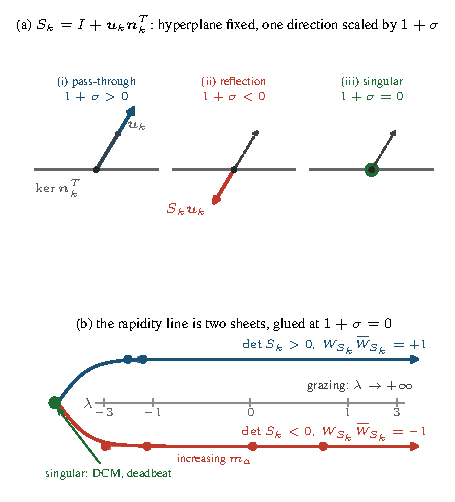
\includegraphics[width=\columnwidth]{figs/geometria_saltacion_rapidez.pdf}
\caption{(a)~A saltation $S_k=I+\bm{u}_k\bm{n}_k^{T}$ fixes the hyperplane
$\ker \bm{n}_k^{T}$ pointwise and scales the crossing direction by
$1+\sigma_k$ (dashed: $\bm{u}_k$; solid: its image); the three types are
the three signs of that factor. (b)~The rapidity
$\lambda=\ln\lvert1+\sigma\rvert$ as a coordinate on two sheets, one per sign
of $\det S_k$, joined at the singular point $1+\sigma=0$ ($\lambda=-\infty$)
and open at $\lambda\to+\infty$. Markers: the traversal of
Table~\ref{tab:especies}, in which a rising compensation ramp drives the
peak event through the singular point at the deadbeat slope $m_a=m_2$.}
\label{fig:geometria}
\end{figure}

For a running example, the $R=15\,\Omega$ current-programmed buck of
Section~\ref{sec:validation} at $D=0.40$ has $m_2/m_1=0.6703$, hence
$1+\sigma=-m_2/m_1=-0.6703$, $\sigma=-1.6703$ and $\lambda=-0.4000$. The
entire saltation lives in the single hyperbolic plane of the current axis,
$\hat{\bm{B}}_S=-\bm{e}^{+}_1\bm{e}^{-}_1$
(recall $2\,\bm{w}_1\!\wedge\!\bm{v}_1=-\bm{e}^{+}_1\bm{e}^{-}_1$), and
\eqref{eq:lift} gives
\begin{equation}
\begin{aligned}
\bm{Q}_S&=1+\tfrac12\sigma\,(1+\hat{\bm{B}}_S)=0.1648-0.8352\,\hat{\bm{B}}_S,\\
\bm{W}_S&=\bm{Q}_S/\sqrt{0.6703}=0.2013-1.0201\,\hat{\bm{B}}_S ,
\end{aligned}
\label{eq:ejemplo}
\end{equation}
which is $-[\sinh(\lambda/2)+\cosh(\lambda/2)\,\hat{\bm{B}}_S]$, the half-turn
form \eqref{eq:halfturn}, with $\bm{W}_S\rev{\bm{W}}_S=-1$.
Equation \eqref{eq:lift} requires no choice of basis or event axis. In the
bucks of Section~\ref{sec:validation} the switching alters one inductor
equation, so $\bm{u}_k$ happens to be axis-aligned; the input-filter platform
of Section~\ref{sec:campana} exercises the general case.

\section{Invariants}
\label{sec:invariants}

\subsection{Rapidity and the Volume Budget}
Each saltation carries the scalar rapidity $\lambda_k=\ln\lvert 1+\sigma_k\rvert$,
computable from the crossing velocities alone. A negative rapidity means that
the event contracts the crossing direction, a positive one that it expands
it. For peak-current control, \eqref{eq:pico} gives it in closed form from
the circuit slopes,
\begin{equation}
\lambda=\ln\left\lvert\frac{m_2-m_a}{m_1+m_a}\right\rvert ,
\label{eq:lampico}
\end{equation}
which reduces to $\ln(m_2/m_1)$ only without a compensation ramp. The ratio
in \eqref{eq:lampico} is the cycle-to-cycle propagation factor of the current
loop in classical sampled-data modeling
\cite{ridley1991new,erickson2020fundamentals}. The algebra adds its status:
the logarithm of that factor is the additive coordinate of a hyperbolic
plane, one coordinate per event, on which the regimes where the sampled-data
factor vanishes or is undefined (the deadbeat slope, DCM, grazing) still
occupy well-defined points or ends.

Rapidities enter the determinant additively. Taking determinants of
\eqref{eq:monodromy},
\begin{equation}
\ln\lvert\det M\rvert=\sum_i \operatorname{tr}(A_{j(i)})\,\tau_i
                      +\sum_k \lambda_k ,
\label{eq:budget}
\end{equation}
an exact contraction budget per cycle in which every interval and every
switching contributes one known scalar; it is the piecewise-smooth form of
Liouville's formula. The additivity is that of $\ln\lvert\det\cdot\rvert$
and not of the algebra. The lifts of different events do not commute, and a
total generator $\log\bm{W}$ need not exist: every exponential of a real
bivector has spinor norm $+1$, while an odd reflection count gives
$\bm{W}\rev{\bm{W}}=-1$. For smooth flows only the first sum exists and
$\det M>0$ always, so the sign structure of a switched converter is carried
by its saltations. Because $\lvert\det M\rvert=\prod_i\lvert\mu_i\rvert$, a
negative budget is necessary for asymptotic stability: the expansion
produced by the saltations must be paid for by the dissipation of the
intervals, $\sum_k\lambda_k<-\sum_i\operatorname{tr}(A_{j(i)})\tau_i$. The
condition certifies instability without any eigenvalue wherever it fails, as
in the first row of Table~\ref{tab:especies} and on the fourth-order platform
of Section~\ref{sec:campana}, but it is not sharp: on the platform of
Section~\ref{sec:ramp} it is violated $0.8$~kA/s before the flip.

\subsection{The Switching-Parity Rule}
\begin{proposition}[Parity]
\label{prop:parity}
Let $M=\Phi_m F_K\Phi_{m-1}\cdots F_1\Phi_0$ be the derivative of the cycle
map of a periodic orbit along which the sequence of events is locally
constant, with $\Phi_i=e^{A_{j(i)}\tau_i}$ and $F_k=I+\bm{u}_k\bm{n}_k^{T}$
nonsingular rank-one factors: saltation matrices of state-triggered events
that are transversal on both sides, $\dot h_k^{-}\neq0$ and
$\dot h_k^{+}\neq0$ (so that every $\lambda_k$ is finite: no event grazes and
none is singular), separated in time from one another and from the clock
edges, with the continuous state not reset at the event; or sample-and-hold
factors of the kind of Section~\ref{sec:retardo}. Let $N_r$ be the number of
factors with $\det F_k<0$---for saltations, the reflection-type events at the
operating point. Then the lift $\bm{W}$ exists and
\begin{equation}
\sgn(\det M)=\bm{W}\rev{\bm{W}}=(-1)^{N_r}.
\label{eq:parity}
\end{equation}
If $N_r$ is odd, $M$ has an odd number of real negative eigenvalues, hence
at least one: the period-doubling channel is open whatever the remaining
parameter values. If $N_r$ is even, the real negative eigenvalues are even
in number, possibly none.
\end{proposition}

\begin{IEEEproof}
$\det e^{A\tau}=e^{\operatorname{tr}A\,\tau}>0$ and $\det F_k=1+\sigma_k$,
which for a saltation is $\dot h_k^{+}/\dot h_k^{-}$ by \eqref{eq:dets},
negative exactly for reflection-type events. By hypothesis no factor is
singular, so $\sgn\det M=(-1)^{N_r}$ by the multiplicativity of the
determinant. Every factor then lies in $GL(n,\mathbb{R})$ and lifts to a
versor, with $\bm{W}_i\rev{\bm{W}}_i=+1$ for rotors and pass-through lifts and
$-1$ for each half-turn \eqref{eq:halfturn} (Proposition~\ref{prop:species});
the spinor norm is multiplicative, so $\bm{W}\rev{\bm{W}}=(-1)^{N_r}$.
Finally, complex eigenvalues occur in conjugate pairs and contribute
$\lvert\mu\rvert^{2}>0$ to $\det M$, and zero is excluded, so $\sgn(\det M)$
is the parity of the number of real negative eigenvalues counted with
multiplicity.
\end{IEEEproof}

\begin{corollary}
\label{cor:n2}
For $n=2$ and odd $N_r$ the spectrum of $M$ is real, one multiplier
negative and one positive: along a branch of orbits with fixed event
itinerary, a second-order converter in the reflection regime can have a
multiplier cross the unit circle only at $-1$ (a flip, or period doubling)
or at $+1$ (a fold), never as a complex pair, which is the Neimark--Sacker
route to a slow oscillation unrelated to the switching period. For even $n$,
odd $N_r$ forces a real positive multiplier as well as a real negative one.
\end{corollary}

Equation~\eqref{eq:parity} follows from the multiplicativity of the
determinant, and neither its matrix form nor its versor form needs an
eigenvalue computation. Under the hypotheses of the proposition, the rule
identifies latched, reflection-type switchings as the only source of
orientation reversal in a converter cycle with continuous state
(Section~\ref{sec:prelim}). The count $N_r$ belongs to the operating point
and changes when an event changes type (Section~\ref{sec:especies}). In
the lift, each reflection contributes a half-turn that moves the monodromy
to the other connected component of the group, which the spinor norm
records. Parameter changes that preserve the type of every event
therefore preserve the parity.

Smooth flows undergo period doubling as well, but their period maps have
positive determinant and cannot force a negative multiplier through
orientation reversal; a transversal Filippov crossing preserves orientation
too (Section~\ref{sec:prelim}). Published data corroborate the rule beyond
our own simulations. The current-mode boost converter of
\cite{parui2002border} has one latched peak-current turn-off per period, so that
$N_r=1$ and \eqref{eq:parity} requires $\det M<0$ on the CCM side; the
Jacobian determinants reported there at two border collisions are $-1.219$
and $-1.588$. Their magnitude exceeds unity, which those
authors flag as ``a possibility which has not been investigated so far'';
the budget \eqref{eq:budget} permits it whenever the saltation rapidities
outweigh the interval contraction. Symmetric two-phase interleaving is a
consistency check in the other direction: there $M=(G\,P_{T/2})^{2}$ with
$G$ the phase-exchange involution, so $\det M>0$ and the orbit belongs to
the even class. Swift and Wiesenfeld prove more in that setting, since the
squaring $\mu_i=\tilde\mu_i^{2}$ makes period doubling of the symmetric orbit
a codimension-two event \cite{swift1984suppression}, but they need the exact
half-period symmetry and a differentiable half-period map. The parity rule
needs neither, and it applies to the mismatched phases of
Section~\ref{sec:validation}, where no such factorization exists.

\subsection{The Grades of the Lift: Flip and Fold as Scalar Zeros}
\label{sec:grades}
The parity rule reads one scalar of the lift, its spinor norm. The remaining
coefficients of the characteristic polynomial of $M$ are scalars of the lift
as well, provided the lift is taken without normalization. Write
$\bm{Q}_{\Phi_i}=e^{\operatorname{tr}(A_{j(i)}\tau_i)/2}\,e^{\bm{B}_{A\tau_i}/2}$
for the interval factors and $\bm{Q}_{S_k}=1+\bm{u}_k\bm{n}_k$ for the
saltations, and let $\bm{Q}_M$ be their ordered product, so that
$\bm{Q}_M\rev{\bm{Q}}_M=\det M$ and $\bm{W}=\pm\bm{Q}_M/\sqrt{\lvert\det M\rvert}$.

\begin{proposition}[Grades of the lift]
\label{prop:grades}
With $\bm{\Gamma}=\prod_{i=1}^{n}\bm{e}^{+}_i\bm{e}^{-}_i$,
\begin{equation}
2^{n}\langle\bm{Q}_M\rangle_0=\det(I+M),\qquad
2^{n}\langle\bm{Q}_M\bm{\Gamma}\rangle_0=\det(I-M),
\label{eq:grades}
\end{equation}
for singular $M$ as well, $\bm{Q}_M$ remaining finite where $\bm{W}$ does not
exist. More generally, with
$\bm{H}(z)=\prod_{i=1}^{n}\bigl[\tfrac12(1+z)+\tfrac12(1-z)\,\bm{e}^{+}_i\bm{e}^{-}_i\bigr]$,
\begin{equation}
2^{n}\langle\bm{Q}_M\bm{H}(z)\rangle_0=\det(I+zM)
\label{eq:charpoly}
\end{equation}
for every $z$, so every coefficient of the characteristic polynomial of $M$
is a scalar part of the lift against a fixed element. Consequently $-1$ is a
Floquet multiplier if and only if $\langle\bm{Q}_M\rangle_0=0$, and $+1$ if
and only if $\langle\bm{Q}_M\bm{\Gamma}\rangle_0=0$; for nonsingular $M$ the
same holds with $\bm{W}$ in place of $\bm{Q}_M$. For $n=2$ the linearized
cycle map is Schur stable if and only if
\begin{equation}
\bm{Q}_M\rev{\bm{Q}}_M<1,\qquad \langle\bm{Q}_M\rangle_0>0,\qquad
\langle\bm{Q}_M\bm{\Gamma}\rangle_0>0 .
\label{eq:jury}
\end{equation}
\end{proposition}

\begin{IEEEproof}
The complete proof is given in Section~S-II of the supplementary material. In
brief: $\Gnn$ with the Witt relations is
the Fock representation on the exterior algebra $\Lambda\mathbb{R}^{n}$,
$\bm{w}_i$ acting by exterior multiplication and $\bm{v}_i$ by contraction;
in it $\bm{Q}_M$ is the exterior-power extension
$\Lambda(M)=\bigoplus_k\Lambda^{k}M$, whose trace is
$\sum_k\operatorname{tr}\Lambda^{k}M=\det(I+M)$ \cite[Sec.~0.8.12]{horn2013matrix},
the scalar part is $2^{-n}$ of the trace, $\bm{\Gamma}$ is the grade involution
$(-1)^{k}$ on $\Lambda^{k}$, and $\bm{H}(z)$ acts as $z^{k}$ on $\Lambda^{k}$.
For $n=2$, \eqref{eq:jury} is the Schur--Cohn test
$1\pm\operatorname{tr}M+\det M>0$, $\lvert\det M\rvert<1$: the two
positivity conditions add to $2(1+\det M)>0$, so with $\det M<1$ they give
$\lvert\det M\rvert<1$.
\end{IEEEproof}

The trace identity is classical. What \eqref{eq:grades}--\eqref{eq:charpoly}
add is that the lifted monodromy carries the whole characteristic polynomial
in its grades, so that the two codimension-one boundaries of a periodic orbit
are zeros of one scalar each, for any $n$ and without eigenvalues. On the
platform of Section~\ref{sec:ramp}, root-finding on
$\langle\bm{Q}_M\rangle_0$ alone locates the subharmonic boundary at
$m_a^{*}=34.038$~kA/s, where the eigenvalues are then found to be
$\{-1,\,0.9675\}$. Near the boundary,
$\langle\bm{W}\rangle_0=\pm(1+\mu_-)(1+\mu_+)/(4\sqrt{\lvert\det M\rvert})$ is
linear in the distance of the flip multiplier from $-1$ and serves as a flip
margin. The proposition also delimits the invariants of the two previous
subsections. The spinor norm and the budget \eqref{eq:budget} fix the sign
and the modulus of $\det M$ and nothing else: the monodromies
$\operatorname{diag}(-0.5,0.5)$ and $\operatorname{diag}(-2,0.125)$ share
reflection count, rapidity and budget, and one is stable while the other is
not. Equation \eqref{eq:grades} supplies the missing coefficients, and it
must be read from the unnormalized lift, because normalizing by
$\sqrt{\lvert\det M\rvert}$ discards the modulus that \eqref{eq:jury} needs
($\tfrac12I$ and $2I$ share every scalar of $\bm{W}$).

The complete chain can be followed on the running example of
Section~\ref{sec:versors}. At $D=0.40$ the inductor-current slopes are
$m_1=74.48$~kA/s and $m_2=49.93$~kA/s, so that $1+\sigma=-m_2/m_1=-0.6703$.
The event is therefore of reflection type, $N_r=1$ and $\lambda=-0.4000$.
The two intervals contribute $\sum_i\operatorname{tr}(A_{j(i)})\tau_i=-0.0180$,
and \eqref{eq:budget} and \eqref{eq:parity} provide
$\det M=-e^{-0.4179}=-0.6584$ before any matrix is multiplied. The lift then
gives $4\langle\bm{Q}_M\rangle_0=\det(I+M)=0.6705$ and
$4\langle\bm{Q}_M\bm{\Gamma}\rangle_0=\det(I-M)=0.0127$. The three conditions
of \eqref{eq:jury} are satisfied and the orbit is stable. The eigenvalues,
$-0.6635$ and $0.9924$, are not required for this conclusion.

\subsection{The Rapidity Sheets: CCM, DCM and the Singular Point}
\label{sec:sheets}
The rapidity of a state-triggered event places the operating regimes of a
converter on one hyperbolic coordinate, though not on one line. Since
$\lambda$ depends on $1+\sigma$ only through its modulus, the sign survives
as a discrete label, and the regimes form the two sheets of
Fig.~\ref{fig:geometria}(b): $\det S_k>0$ with
$\bm{W}_{S_k}\rev{\bm{W}}_{S_k}=+1$, and $\det S_k<0$ with
$\bm{W}_{S_k}\rev{\bm{W}}_{S_k}=-1$. The sheets are joined at one point, the
singular value $1+\sigma=0$, and open at $\lambda\to+\infty$, which is
reached when $\dot h^{-}\to0$ with $\dot h^{+}$ fixed; the trajectory then
grazes the switching surface and the saltation ceases to exist. The sheet
label of an event can change through either end. In peak-current control
$\dot h^{-}=m_1+m_a>0$, so only the singular point is available, and
Section~\ref{sec:especies} passes through it with the compensation ramp. An
orbit's total $\bm{W}\rev{\bm{W}}$ is the product of the sheet labels of its
events, and to change it one event must change sheet. Two cautions apply at
the open end. The rapidity measures the signed volume scaling of a saltation
and not its shear. Moreover, with a ramp the peak event cannot graze, since
$\dot h^{-}\geq m_a$; the sweep of Section~\ref{sec:sweep} approaches
$\lambda\to+\infty$ with $m_a=0$ as $D\to1$, where the peak event also
approaches the clock edge.

At the zero-current event of DCM, $\dot h^{+}=0$ identically, so $1+\sigma=0$
and the saltation is singular, of type~(iii): one Floquet multiplier is
exactly zero and $\lambda=-\infty$ is the infinitely stabilizing end of the
sheets, where the lift leaves the group. This is a second event, distinct
from the peak turn-off, whose own rapidity stays finite throughout DCM
($\lambda=-2.27$ at $I_{\mathrm{ref}}=0.10$~A on the platform of
Section~\ref{sec:sweep}). In the buck the projector is
$\operatorname{diag}(0,1,\dots)$, because at $i_L=0$ the capacitive rows of
$\bm{f}^{+}$ and $\bm{f}^{-}$ coincide and the field jump is parallel to
$\bm{n}_k$; in general $S_k$ is an oblique projector along $\bm{u}_k$.

The DCM orbit also shows why the hypothesis of Proposition~\ref{prop:parity}
cannot be dropped. It has one latched peak turn-off, so $N_r=1$ is odd, yet
$\det M=0$: the sign predicted by \eqref{eq:parity} is not attained, and
Section~\ref{sec:validation} finds no real negative multiplier there. The
singular event overrides the parity. The override is not a general rule,
since $\det M=0$ does not by itself preclude real negative multipliers; it
is a property of this orbit. With $n=2$,
$M=\Phi_{\mathrm{idle}}\,\operatorname{diag}(0,1)\,\Phi_{\mathrm{off}}
S_{\mathrm{peak}}\Phi_{\mathrm{on}}$ has a single nonzero multiplier, the
derivative of the reduced voltage map: the projector removes the current
component at the zero-current instant and only the voltage contribution
survives, with a value near $+0.99$ across the DCM band of
Fig.~\ref{fig:rapidity}. Continuous conduction spans the finite part of the
sheets and crosses $\lambda\approx 0$ near the flip boundary. The CCM--DCM
transition is a border collision at which the cycle gains or loses an entire
interval, and the flip multiplier jumps to zero. This is the change of state-space
dimension identified in \cite{parui2002border}, where the map is
two-dimensional in CCM and one-dimensional in DCM. In the present language
the rank drop is the entry of a singular event into the itinerary.
The resulting one-sided rank deficiency is the zero-determinant regime of
the border-collision normal form \cite{simpson2025zero,fatoyinbo2023synopsis}.

The correspondence with the classification of piecewise-linear maps can now
be stated explicitly. In the two-dimensional normal form the map on each
side of the border is characterized by a trace and a determinant,
$(\tau_L,\delta_L)$ and $(\tau_R,\delta_R)$, and a side is
orientation-preserving, orientation-reversing or noninvertible for
$\delta>0$, $\delta<0$ or $\delta=0$, respectively
\cite{ghosh2025robust,simpson2025zero}. In the present terms $\delta$ is
$\det M$ on that side. Its sign is $(-1)^{N_r}$ by \eqref{eq:parity}, and
$\delta=0$ corresponds to a singular event in the itinerary, so that the two
classifications coincide. The difference lies in the origin of the numbers.
The normal form takes them as parameters of a map that has already been
extracted, whereas here the sign follows from a count of circuit events, the
modulus from \eqref{eq:budget} and the trace from \eqref{eq:grades}. At the
CCM--DCM border of the platform of Section~\ref{sec:sweep}, for instance, the
lift gives $(\tau_L,\delta_L)=(0.8666,-0.1216)$ on the CCM side, where
$N_r=1$, and $(\tau_R,\delta_R)=(0.9895,0)$ on the DCM side, where the
zero-current event is singular. Both sides are attracting and the fixed
point persists across the border, in agreement with
Fig.~\ref{fig:rapidity}. The algebra thus adds no new class to the
orientation classification. It supplies the event-level origin of each
class and the values of the parameters.

\section{Simulation Study on Realistic Converter Models}
\label{sec:validation}
All studies use a 12-V, 100-kHz buck platform with $L=100\,\mu\mathrm{H}$,
$C=100\,\mu\mathrm{F}$, conduction losses ($R_L=60\,\mathrm{m}\Omega$,
$R_{on}=40\,\mathrm{m}\Omega$), capacitor ESR ($25\,\mathrm{m}\Omega$) and a
diode model ($V_d=0.45$~V, $R_d=20\,\mathrm{m}\Omega$), so that
$A_{\mathrm{on}}\neq A_{\mathrm{off}}$ throughout. Three load conditions are
used: $R=3\,\Omega$ with $I_{\mathrm{ref}}=3.35$~A (Section~\ref{sec:ramp}),
$R=1.5\,\Omega$ for the interleaved converters (Section~\ref{sec:ident}), and
$R=15\,\Omega$ for the light-load sweep (Section~\ref{sec:sweep}). Where a
study departs from this platform (input filter, parallel modules, digital
loop) its parameters are stated with it. On the buck and interleaved
platforms of Sections~\ref{sec:ramp}--\ref{sec:especies} the versor action
reproduces every monodromy matrix to machine precision, $\le 7\times10^{-16}$
in the largest entry.

\subsection{Exact Subharmonic Boundary Versus the Classical Ramp Rule}
\label{sec:ramp}
We first ask whether the flip boundary predicted by the lift is the one a
time-domain simulation shows, and how far it lies from the textbook ramp
rule once losses are included. The exact boundary, located by $\mu=-1$ on
the versor monodromy or equivalently by $\langle\bm{Q}_M\rangle_0=0$, lies
at $m_a^{*}=34.04$~kA/s, where the duty cycle is $D=0.7767$. The classical
sampled-data boundary is $\alpha=-(m_2-m_a)/(m_1+m_a)=-1$, that is,
$m_a=(m_2-m_1)/2$ \cite{ridley1991new,erickson2020fundamentals}. Because the
slopes move with the ramp, its self-consistent prediction is the root of
$m_a=[m_2(m_a)-m_1(m_a)]/2$, at $34.34$~kA/s; the rule evaluated on the exact
boundary orbit gives $34.41$~kA/s. The two conditions differ: at $m_a^{*}$
the peak-event rapidity is $\lambda=+0.0121$, not zero, and by
\eqref{eq:lampico} $\lambda=0$ is the classical rule itself. In the lossless
limit all three coincide to $0.003\%$. Losses open a gap of
$0.30$--$0.37$~kA/s, and the budget gives it in closed form. At a flip of a
second-order converter $\det M=-\mu_+$, so \eqref{eq:budget} on the boundary
orbit reads
\begin{equation}
\lambda^{*}=\ln\mu_+-\sum_i\operatorname{tr}(A_{j(i)})\tau_i
=-0.0330+0.0451=+0.0121,
\label{eq:gap}
\end{equation}
and with $\kappa=e^{\lambda^{*}}$ the boundary is
$m_a^{*}=(m_2-\kappa m_1)/(1+\kappa)$. The classical rule is the case
$\kappa=1$, in which the voltage multiplier equals the Liouville factor
$e^{\sum\operatorname{tr}A\tau}$; the gap to the rule evaluated on the same
orbit is $\tfrac12(m_1+m_2)\tanh(\lambda^{*}/2)=0.374$~kA/s. Since $m_1$,
$m_2$ and $\mu_+$ belong to the boundary orbit, \eqref{eq:gap} explains the
gap rather than predicting the boundary.

Resolving a gap of $0.3$~kA/s requires care. The ramp slope at which the
subharmonic visually disappears in a bifurcation diagram is not usable,
because the period-2 amplitude vanishes continuously at a flip and
convergence there is marginal. The amplitude itself was therefore computed.
An event-driven
simulation, independent of the Floquet construction and using bisected
crossing instants, is run under parameter continuation on a fine grid inside
the window $33.35$--$34.02$~kA/s, where the attractor is a verified clean
two-cycle (36 of 40 points; below $33.3$~kA/s the orbit has higher period or
is chaotic). For a supercritical flip the squared amplitude is
asymptotically linear in the parameter, and it is, with $R^{2}=0.99991$ over
the window. Extrapolating to zero places the boundary at
\begin{equation}
m_a^{\mathrm{meas}}=34.045\pm0.001~\mathrm{kA/s},
\end{equation}
which agrees with the versor prediction to $0.02\%$ and misses the
self-consistent classical boundary by forty times that amount
(Fig.~\ref{fig:bifurcation}). The residual $7$~A/s offset from $m_a^{*}$
exceeds the statistical uncertainty of the fit and is systematic, as
expected from a finite extrapolation window in which the asymptotic law is
only approached; it does not affect the discrimination.

\begin{figure}[!t]
\centering
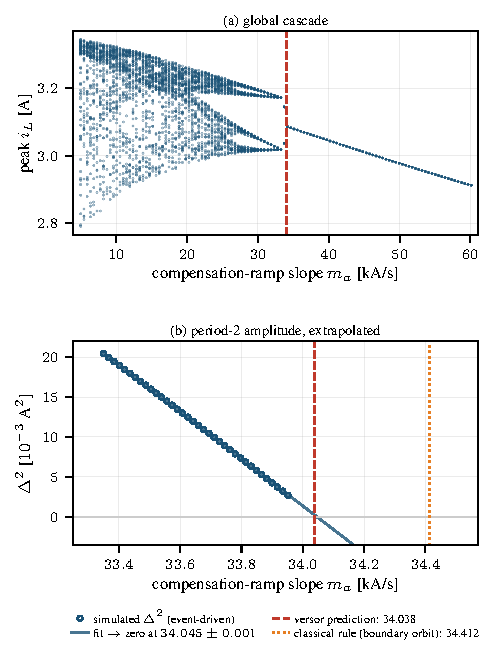
\includegraphics[width=\columnwidth]{figs/bifurcacion_buck_realista.pdf}
\caption{Subharmonic boundary of the lossy buck ($R=3\,\Omega$,
$I_{\mathrm{ref}}=3.35$~A; $D$ runs from $0.838$ to $0.730$ across the
sweep). (a)~Peak inductor current of the attractor over a wide ramp sweep,
sampled once per cycle after 400 transient cycles; the $0.46$~kA/s grid of
this overview cannot resolve the gap between the candidate boundaries.
(b)~Squared period-2 amplitude $\Delta^{2}$ (circles) computed by the
event-driven simulator under continuation, restricted to verified
two-cycles, with its linear least-squares fit ($R^{2}=0.99991$) extrapolated
to zero. The zero crossing falls on the versor prediction (dashed) and
excludes the classical rule evaluated on the boundary orbit (dotted; its
self-consistent root lies at $34.34$~kA/s).}
\label{fig:bifurcation}
\end{figure}

\subsection{Independent Identification of the Monodromy}
\label{sec:ident}
Interleaved converters run $N$ identical phases into one capacitor with
clocks staggered by $T/N$. Two- and three-phase versions of the platform
share the output capacitor ($C=100\,\mu$F, ESR $25\,\mathrm{m}\Omega$) and
drive $R=1.5\,\Omega$, with tolerance-level mismatch between phases: for
$N=2$, $L=100/106\,\mu$H with $R_L=60/52\,\mathrm{m}\Omega$ and
$I_{\mathrm{ref}}=1.60$~A; for $N=3$, $L=100/104/97\,\mu$H with
$R_L=60/55/65\,\mathrm{m}\Omega$ and $I_{\mathrm{ref}}=0.86$~A. Each phase
carries its own latched peak comparator, and the duty cycles are $D=0.397$
and $D=0.305$. We identified the monodromy from a time-domain simulator with
the real latch logic by least-squares fitting of cycle-to-cycle perturbation
data, a route independent of the Floquet construction. The simulator advances
with a fixed step $T/2100$ and locates each comparator crossing by linear
interpolation within the step. After $260$ transient cycles the orbit is
perturbed by $\pm10$~mA on each phase current and $\pm50$~mV on $v_C$, $13$
cycles are recorded per perturbation at the phase-1 clock, and $M$ is the
least-squares solution of $Y=MX$ over the transition pairs.
Table~\ref{tab:ident} compares the two routes.

\begin{table}[!t]
\caption{Predicted versus identified Floquet multipliers of the interleaved
converters with component mismatch. ``V'' is the versor prediction, ``I''
the least-squares identification from the independent time-domain
simulator. Entries are rounded to four decimals; the largest discrepancy
over all entries is $8.7\times10^{-5}$ in modulus ($8.2\times10^{-5}$ in any
real or imaginary part).}
\label{tab:ident}
\centering
\setlength{\tabcolsep}{4pt}
\begin{tabular}{@{}llcc@{}}
\toprule
& & 2 phases ($N_r=2$) & 3 phases ($N_r=3$) \\
\midrule
\multirow{2}{*}{flip pair}
  & V & $-0.6542\pm0.0015j$ & $-0.4359\pm0.0019j$ \\
  & I & $-0.6542\pm0.0015j$ & $-0.4358\pm0.0020j$ \\[2pt]
\multirow{2}{*}{real flip}
  & V & --- & $-0.4357$ \\
  & I & --- & $-0.4356$ \\[2pt]
\multirow{2}{*}{voltage}
  & V & $0.9348$ & $0.9314$ \\
  & I & $0.9348$ & $0.9314$ \\[2pt]
\multirow{2}{*}{$\det M$}
  & V & $+0.4001$ & $-0.0771$ \\
  & I & $+0.4001$ & $-0.0771$ \\[2pt]
$\bm{W}\rev{\bm{W}}$ & & $+1$ & $-1$ \\
\bottomrule
\end{tabular}
\end{table}

\subsection{The Parity Rule Under Broken Symmetry}
Table~\ref{tab:ident} and Fig.~\ref{fig:parity} show
Proposition~\ref{prop:parity} at work. With three mismatched phases $N_r=3$
is odd, so a real negative multiplier is forced, and one appears at
$-0.4357$ next to a complex flip pair; $\det M<0$ and
$\bm{W}\rev{\bm{W}}=-1$. With two phases $N_r=2$ is even, the determinant is
positive, and no real negative multiplier is present: the would-be flip pair
is complex, close to the negative axis at
$\operatorname{Im}\mu=\pm1.5\times10^{-3}$. The asymmetry between the two
cases is the content of the rule. The odd case is forced. The even case is
only permitted, since a pair of real negative multipliers would be equally
admissible, and Section~\ref{sec:par} determines which of the two occurs.
Mismatch of this order is
unavoidable in parallel-connected converters, whose bifurcation behavior has
been studied in this journal \cite{iu2001bifurcation}.

\begin{figure}[!t]
\centering
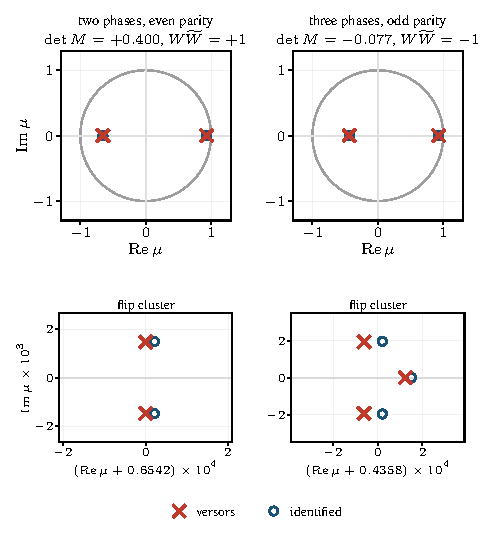
\includegraphics[width=\columnwidth]{figs/paridad_interleaved_realista.pdf}
\caption{Floquet multipliers of the interleaved converters: versor
prediction (crosses) and independently identified values (circles). Left
column, two phases, even parity; right column, three phases, odd parity.
Top row, the unit circle. Bottom row, the flip cluster magnified, with the
real and imaginary axes scaled by $10^{4}$ and $10^{3}$ because the two
spreads differ by an order of magnitude. With two mismatched phases the flip
multipliers form a complex pair off the real axis; the third phase adds a
real negative multiplier next to the pair.}
\label{fig:parity}
\end{figure}

\subsection{The Even Case: Interference of Two Reflections}
\label{sec:par}
For an even count, Proposition~\ref{prop:parity} permits a pair of real
negative multipliers but does not force it. In the two-phase converter the
alternative can be decided. The switching of phase $k$ modifies the equation
of the corresponding inductor only. Hence, $S_k$ differs from the identity
in one diagonal entry, $1+\sigma_k$, and the two phases interact through the
output capacitor and the ESR, $r_C$. To first order in that interaction, the
flip pair consists of the eigenvalues of
\begin{equation}
\begin{bmatrix}\mu_1 & \chi_1\\ (1+\sigma)\chi_2 & \mu_2\end{bmatrix},
\qquad \mu_k=(1+\sigma_k)\,e^{-\rho_k},
\label{eq:bloque}
\end{equation}
where $\mu_k$ is the flip multiplier that phase $k$ would have with a stiff
output and $\rho_k$ is the series resistance of phase $k$ divided by $L_k$
and integrated over one period. The entry $\chi_k$ is the perturbation
induced in the current of phase $k$ by the other phase over half a period,
and the closed form is given in Section~S-VIII of the supplementary
material. The pair is given by
\begin{equation}
\begin{aligned}
\mu_{\pm}&=\tfrac12(\mu_1+\mu_2)\pm\sqrt{\tfrac14(\Delta\mu)^{2}-\chi^{2}},\\
\Delta\mu&=\mu_1-\mu_2,\qquad \chi^{2}=-(1+\sigma)\,\chi_1\chi_2 .
\end{aligned}
\label{eq:par}
\end{equation}
The sign of $\chi^{2}$ is that of the event type. Two reflection-type events
have $1+\sigma<0$ and hence $\chi^{2}>0$, and the interaction separates the
pair off the real axis. On the other hand, for two pass-through events $\chi^{2}<0$ and the same
interaction separates the pair along the axis, as was verified by raising
the ramp beyond the deadbeat slope (Section~S-VIII). Therefore, with
two reflections the pair is complex if and only if
$\lvert\Delta\mu\rvert<2\chi$. At the subharmonic boundary, where
$\lvert1+\sigma\rvert\approx1$,
\begin{equation}
\chi=\frac{\gamma^{2}T^{2}}{4C\sqrt{L_1L_2}}
=\gamma^{2}\left(\frac{\pi f_0}{f_s}\right)^{2},
\label{eq:chi0}
\end{equation}
where $\gamma=R/(R+r_C)$, $f_0$ is the resonant frequency of one inductance
with the output capacitor and $f_s=1/T$. As a consequence, a two-phase
converter whose reflections differ by less than $2\chi$ loses stability
through a Neimark--Sacker bifurcation, in which the subharmonic is modulated
at the frequency $f_s\sqrt{\chi^{2}-(\Delta\mu)^{2}/4}/(2\pi)$. Otherwise it
undergoes a period doubling, which is dominated by the phase with the larger
$\lvert\mu_k\rvert$. In the lift, the composition of the two half-turn
versors \eqref{eq:halfturn} with the flows is elliptic in the first case and
hyperbolic in the second.

The criterion was tested on the two-phase platform of
Section~\ref{sec:ident}. In particular, at the operating point of
Table~\ref{tab:ident} the closed forms give $\lvert\Delta\mu\rvert/2\chi=0.55$ and an imaginary
part of $1.49\times10^{-3}$, compared with $1.474\times10^{-3}$ from the
monodromy matrix. With a compensation ramp of $10$~kA/s the stability
boundary is located at $D=0.58$, where \eqref{eq:chi0} gives
$\chi=2.42\times10^{-3}$. The threshold $2\chi$ then amounts to $0.48\%$ of
$\lvert1+\sigma\rvert$, and the modulation frequency for equal phases is
$38.5$~Hz. An event-driven simulation in the time domain, which uses no
saltation matrix, was run $1$~mA beyond the boundary for $17$ values of
$L_2/L_1$ (Fig.~\ref{fig:par}). With equal phases the subharmonic is
modulated with a period of $2634$ switching cycles, compared with $2598$
from \eqref{eq:chi0}. The modulation frequency decreases with the mismatch
according to \eqref{eq:par} and vanishes between $L_2/L_1=1.0150$ and
$1.0155$, where \eqref{eq:par} predicts $1.0153$. Beyond that value the
attractor is a period-two orbit. The same classification was obtained in
$48$ further runs, with eight mismatches of $L$ and $R_L$ at distances of up
to $20$~mA from the boundary. It should be noted that, without a ramp,
$1+\sigma=-m_2/m_1$ does not depend on the inductance, and a mismatch of
$10\%$ leaves the pair complex.

\begin{figure}[!t]
\centering
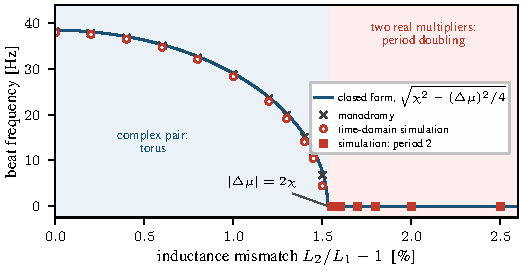
\includegraphics[width=\columnwidth]{figs/par_flip_dos_fases.pdf}
\caption{The even case in the two-phase converter, $1$~mA beyond the
stability boundary ($m_a=10$~kA/s, $D=0.58$). Modulation frequency of the
subharmonic against the inductance mismatch: closed form \eqref{eq:par},
monodromy matrix and time-domain simulation. The modulation vanishes at
$\lvert\Delta\mu\rvert=2\chi$.}
\label{fig:par}
\end{figure}

Published data are consistent with this result. The two-phase boost
converter of \cite{giaouris2013foldings} has equal phases and no ramp, and
the period-one orbit loses stability with the pair $-0.9994\pm0.0349j$. This
is described there as a Neimark--Sacker bifurcation with features of a
period doubling that had not been reported in power converters. The
monodromy matrix of that converter, computed as in Section~\ref{sec:prelim},
reproduces the published multipliers within the four digits printed
(Table~S9). Both events are of reflection type, and the reduction
\eqref{eq:bloque}, evaluated numerically, gives $\chi=0.037$. The pair is
therefore complex for $\lvert\Delta\mu\rvert<0.073$, and in the absence of a
ramp an inductance mismatch of $20\%$ does not leave this window.

\subsection{One Sweep Across the Rapidity Sheets}
\label{sec:sweep}
Fig.~\ref{fig:rapidity} sweeps the current reference of the light-load
platform ($R=15~\Omega$, $m_a=0$) from deep DCM to near duty saturation. The
boundary values quoted here are roots located by bisection on the versor
monodromy, not grid points. At this load the conduction parameter
$2L/(RT)=1.33$ exceeds unity, so an ideal buck would stay in CCM at every
duty cycle; the DCM band exists because the diode drop is comparable to the
output ($v_o=0.91$~V at the border). Since the sweep varies $I_{\mathrm{ref}}$
at fixed load, $v_o$ runs from $0.9$ to $11.7$~V across it. The flip
multiplier is exactly zero throughout DCM, where the singular zero-current
event of type~(iii) makes $\det M=0$ although $N_r=1$ is odd, and it
jumps to $-0.1229$ at the border, which lies at
$I_{\mathrm{ref}}^{*}=0.12158$~A ($D=0.1097$, where the valley current
reaches zero). It then descends through $-1$ at $I_{\mathrm{ref}}=0.53944$~A,
that is, at $D=0.50144$: the lossy model reproduces the classical half-duty
rule to within $0.29\%$. Beyond that point the rapidity climbs to $+4.1$ at
$D=0.984$ as the peak event approaches the clock edge
(Section~\ref{sec:invariants}).

\begin{figure}[!t]
\centering
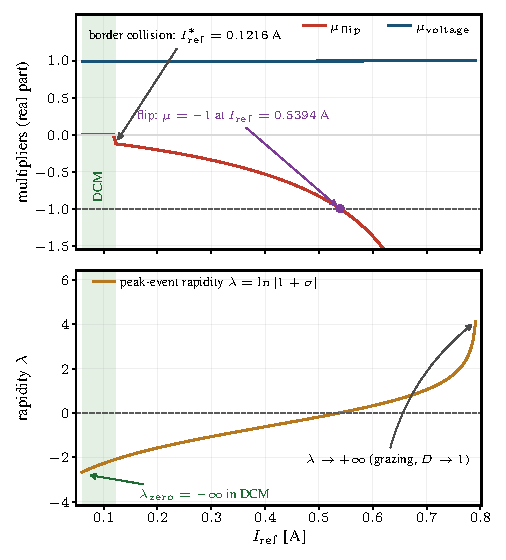
\includegraphics[width=\columnwidth]{figs/recta_rapidez_ccm_dcm_grazing.pdf}
\caption{The $R=15\,\Omega$ platform with $I_{\mathrm{ref}}$ swept from DCM
(shaded) to near duty saturation, $m_a=0$. Top: real parts of the
multipliers; the flip multiplier is identically zero in DCM, jumps to
$-0.1229$ at the border $I_{\mathrm{ref}}^{*}=0.1216$~A and crosses $-1$
(marker) at $0.5394$~A. Bottom: rapidity of the peak event, finite
throughout; the zero-current event of DCM carries $\lambda=-\infty$.}
\label{fig:rapidity}
\end{figure}

\subsection{Traversing the Three Event Types With One Parameter}
\label{sec:especies}
Section~\ref{sec:prelim} claimed that the type of an event belongs to the
operating point and not to the detector. Table~\ref{tab:especies} tests the
claim on the $R=3\,\Omega$ platform of Section~\ref{sec:ramp} with the peak
comparator and latch untouched. Only $m_a$ varies, and $m_2$ is recomputed at
each point because the periodic orbit moves with the ramp.

\begin{table}[!t]
\caption{The latched peak event traverses the three saltation types as the
compensation ramp is raised on one power stage ($R=3\,\Omega$,
$I_{\mathrm{ref}}=3.35$~A). The singular row is the deadbeat condition
$m_a=m_2$, where one multiplier vanishes and no versor represents the
saltation.}
\label{tab:especies}
\centering
\setlength{\tabcolsep}{3.5pt}
\begin{tabular}{@{}rrrrl@{}}
\toprule
$m_a$ [kA/s] & $m_2$ [kA/s] & $1+\sigma$ & $\det M$ & type \\
\midrule
$20.00$ & $99.84$ & $-1.8137$ & $-1.734$   & reflection \\
$34.04$ & $96.35$ & $-1.0122$ & $-0.968$   & reflection ($\mu=-1$) \\
$60.00$ & $90.57$ & $-0.3275$ & $-0.313$   & reflection \\
$80.00$ & $86.61$ & $-0.0564$ & $-0.054$   & reflection \\
$85.58$ & $85.58$ & $\ \ \ 0$ & $\ \ \ 0$  & \textbf{singular} (deadbeat) \\
$110.00$ & $81.34$ & $+0.1878$ & $+0.180$  & pass-through \\
$130.00$ & $78.19$ & $+0.2947$ & $+0.282$  & pass-through \\
\bottomrule
\end{tabular}
\end{table}

The traversal is drawn on the sheets of Fig.~\ref{fig:geometria}(b). Three
things follow. First, $N_r$ for this circuit is $1$ below $m_a=85.58$~kA/s
and $0$ above it, so the parity of \eqref{eq:parity} changes with a control
setting; the reflection count is a datum of the operating point, and
Proposition~\ref{prop:parity} must be read at a point, not at a topology.
The change is the passage between sheets, and it is unavoidable: to reach
pass-through from reflection the event must become a projector on the way.
Second, the deadbeat slope is the type boundary. The condition $m_a=m_2$
is classical; in the frozen-output, constant-slope model of the current loop
it corrects a current perturbation in one cycle
\cite{ridley1991new,erickson2020fundamentals}. In the full two-state model it
means that the saltation has become a projector, with rapidity $-\infty$,
and what is annihilated in one cycle is the perturbation along
$\ker M=\Phi_{\mathrm{on}}^{-1}\ker S$, a direction with a small voltage
component. A pure current perturbation is not annihilated ($Me_i\neq0$), and
the switching function does not stay clamped afterwards: $\dot h^{+}=0$ at
the instant and $\ddot h^{+}\neq0$ a moment later. Third, the sign of
$\det M$ tracks the type with no eigenvalue computation, including
through the zero, where every eigenvalue-based criterion is least well
conditioned.

The deadbeat identification admits a check in the time domain. Since
$\det S=0$ makes $M$ rank-deficient, one direction of perturbation must be
annihilated to first order in a single period. When the periodic orbit is
perturbed along $\ker M$ and one cycle is integrated with an event-driven
solver, the residual scales as the square of the perturbation over three
decades, $\delta=10^{-2}$ to $10^{-5}$, with a log--log slope of $2.0000$.
The linear part is therefore annihilated, and the remainder is the
second-order term of the nonlinear cycle map.

\subsection{Converters of Different Structure and Modeling Detail}
\label{sec:otros}
The platforms considered so far share the buck power stage and the latched
peak comparator. Two converters of different structure were therefore
analyzed. The first is the voltage-mode buck converter of
\cite{deane1990instability,fossas1996study,giaouris2008stability}
($L=20$~mH, $C=47\,\mu$F, $R=22\,\Omega$, $T=400\,\mu$s), in which the switch
is closed while the amplified output error is below a sawtooth ramp and no
latch is present. The switching function depends on the capacitor voltage
only and the switching modifies the inductor equation only, so that
$\bm{n}^{T}(\bm{f}^{+}-\bm{f}^{-})=0$. The event is pass-through with
$\sigma=0$, $N_r=0$, and \eqref{eq:budget} gives $\det M=e^{-T/(RC)}=0.6792$
at every operating point. As a consequence, the Floquet multipliers remain
on the circle of radius $e^{-T/(2RC)}=0.8241$ while they are complex, reach
the real axis at $V_{\mathrm{in}}=24.086$~V and then separate with a constant
product. The period doubling of this converter thus occurs with two real
negative multipliers, which is the case that Proposition~\ref{prop:parity}
permits but does not force. The multipliers listed in Table~I of
\cite{giaouris2008stability} for $V_{\mathrm{in}}=14$, $20$, $24$ and $25$~V
are reproduced within the four digits printed there, and their products agree with $0.6792$ within the printed precision in the
four rows, although this invariant is not stated in
\cite{giaouris2008stability}. The zero of $\langle\bm{Q}_M\rangle_0$ locates
the flip boundary at $V_{\mathrm{in}}^{*}=24.517$~V, with multipliers
$\{-1,\,-0.6792\}$. A time-domain simulation with the modulator logic
provides $24.513$~V, and the experimental waveforms of
\cite{giaouris2008stability} show a period-one orbit at $20$~V and a
period-two orbit at $25$~V.

The second converter is a boost converter under peak-current control
($V_{\mathrm{in}}=5$~V, $R=10\,\Omega$, $I_{\mathrm{ref}}=3$~A, with the
passive and parasitic elements of the buck platform). In this topology the
switching modifies both state equations, and the normalized field jump is
not aligned with a coordinate axis even for $n=2$. At $m_a=60$~kA/s,
$\bm{u}=[-1.0365,\,0.2467]^{T}$ and
$1+\sigma=\dot h^{+}/\dot h^{-}=-0.0365$, so that the event is of reflection
type, $N_r=1$ and $\det M=-0.0357$. The zero of $\langle\bm{Q}_M\rangle_0$
locates the flip boundary at $m_a^{*}=11.2663$~kA/s ($D=0.5965$), and the
closed form of Section~\ref{sec:ramp}, $m_a^{*}=(m_2-\kappa m_1)/(1+\kappa)$,
returns the same value. The time-domain simulation with the latch logic
provides $11.2664$~kA/s from twelve verified two-cycles. On this platform
$\lambda^{*}=1.1\times10^{-4}$, because the voltage multiplier almost
coincides with the Liouville factor, and the classical rule deviates by
$0.03\%$ only. The gap of about $1\%$ found for the buck converter is
therefore a property of the operating point, which \eqref{eq:gap}
quantifies.

Finally, the dependence of $N_r$ on the level of modeling detail was
examined on the platform of Section~\ref{sec:ramp} at $m_a=50$~kA/s. A
first-order current-sensing filter with corner frequency $f_f$ was placed
ahead of the comparator. With ideal sensing,
$1+\sigma=-0.526$, $N_r=1$ and the multipliers are $\{-0.5205,\,0.9660\}$.
With the filter, $\det S=1$ for every $f_f$ between $0.5$ and $50$ times the
switching frequency, because the derivative of the filtered current does not
jump at the switching; hence $N_r=0$ and $\det M>0$. The flip multiplier
remains at $-0.5263$ for $f_f=5/T$ and at $-0.5210$ for $f_f=50/T$, and it is
accompanied by a real negative multiplier of order $e^{-2\pi f_fT}$, which
restores the even parity. The prediction of the reduced model is thus
preserved, while the orientation reversal is transferred from the event to
the sensing dynamics, as to the sampler of Section~\ref{sec:retardo}.

\subsection{Numerical Verification of the Lift and Its Conditioning}
\label{sec:campana}
The results above are individual operating points. The identities behind
them were also checked in bulk on $2\times10^{4}$ random switched systems
with $n=2,\dots,8$ (supplementary Section~S-VII). The closed form for
$\det M$, the assembled product and the parity of the real negative
multipliers agreed in every case, as a proved identity must. In $24\%$ of
the trials an even $N_r$ came with two or more real negative multipliers, so
that the permissive half of Proposition~\ref{prop:parity} describes a common
configuration.

The cost and the accuracy of the lift depend on how the versor is stored
(supplementary Tables~S1--S3). A general element of $\Gnn$ has $4^{n}$
coefficients, but this dimension is never required. A versor is a product
of vectors and can be stored as the list of its factors, which belong to the
$2n$-dimensional space, and a composition is then a concatenation. A
saltation with $\sigma_k\neq0$ contributes exactly two factors,
$\bm{u}_k+\bm{n}_k$ and $\bm{u}_k/\sigma_k+(1+1/\sigma_k)\bm{n}_k$, with
squares $\sigma_k$ and $(1+\sigma_k)/\sigma_k$, which have opposite signs for
a reflection-type event. In this form the complete cycle requires about ten
times the multiplications of the $n\times n$ route for every $n$ from $2$ to
$8$, which is a constant factor. With a numerical library that implements
this representation \cite{eid2025gafl}, the factored versor reproduced $M$
within $1.2\times10^{-14}$ for $n\le7$ and $8\times10^{-13}$ for $n=8$, and
the sign of $\det M$ read from the factors was correct in all cases. The
accuracy is maintained near the degenerate types: the median error remains
at $3\times10^{-15}$ for $10^{-10}\le\lvert1+\sigma\rvert\le10^{10}$ and for
$\lvert\sigma\rvert\ge10^{-10}$. Closer to the singular and parabolic values
one factor becomes a null vector and the library rejects the factorization,
in agreement with Proposition~\ref{prop:species}. The loss of accuracy that
was reported in the first version of this paper for the normalized versor
was therefore a property of the generic multivector implementation. It
reappears, with errors of order one at $\lvert1+\sigma\rvert=10^{-8}$, when
the factored versor is assembled into the $2n\times2n$ matrix of its action
and factored again, which indicates that the versor should be kept in
factored form. The matrix route is equally accurate and is faster by the
constant factor above. The count is not affected by any of these choices:
once the type of every event is known, $N_r$ is an integer and
\eqref{eq:parity} gives $\sgn(\det M)$ whatever the conditioning.

A fourth-order platform exercises the general closed form. A buck converter
preceded by an input $LC$ filter ($L_f=47\,\mu$H, $C_f=22\,\mu$F,
$R_{L_f}=30\,\mathrm{m}\Omega$, no capacitor ESR, $m_a=0$;
$\bm{x}=[i_{L_f},v_{C_f},i_L,v_C]^{T}$) has a switching that alters both the
filter-capacitor and the inductor equations, so that
$\bm{u}_k=[0,\,9.190,\,-7.364,\,0]^{T}$ is aligned with no axis. The versor
reproduces the saltation to $8.9\times10^{-15}$ and the monodromy to a
relative $2.1\times10^{-15}$. The event is of reflection type with
$1+\sigma=-6.364$, so that $N_r=1$ and \eqref{eq:parity} forces $\det M<0$;
the computation returns $-6.0575$ and the budget \eqref{eq:budget} closes to
$4\times10^{-16}$. The filter is deliberately undamped and violates
Middlebrook's criterion \cite{middlebrook1976}, and is not a design. It also shows what the parity rule does not
decide. At the flip boundary, $m_a^{*}=32.64$~kA/s, the
multipliers are $\{-1,\,0.967,\,0.994\pm0.316j\}$: the complex pair has
modulus $1.044$, and the flip that \eqref{eq:parity} governs is not the
binding constraint.

Published data extend the check to topologies that were not simulated here.
Table~\ref{tab:literatura} collects the studies that report Floquet
multipliers of a switched converter with enough detail to count $N_r$ from
the switching logic. Every entry is consistent with \eqref{eq:parity}: odd
counts come with a real negative multiplier, the even count keeps the flip
pair complex \cite{giaouris2013foldings}, and a count of zero forces none
\cite{dranga2003stability}. In the fifth-order resonant converter of
\cite{dranga2003stability} the two state-triggered turn-offs are
pass-through with $\det S_k=+1$, the instability reported is a Hopf crossing
of a complex pair, and the multipliers printed belong to the
symmetry-reduced half-period map, which does not affect the parity
statement. This is corroboration and not a proof, since $N_r$ was inferred
from the switching logic as described by each source.

\begin{table}[!t]
\caption{Published multipliers of switched converters against the parity
rule. $N_r$ is counted here from the switching logic each source describes
(latched peak comparators in \cite{parui2002border,imrayed2013controlling,
giaouris2013foldings,hayes2020application}, pass-through turn-offs in
\cite{dranga2003stability}); the multipliers are as printed by those sources,
at $I_{\mathrm{ref}}=0.1$~A for \cite{giaouris2013foldings}; $\dagger$:
eigenvalues of the symmetry-reduced half-period map; $\ddagger$: the source
prints an imaginary part of $0.0014$ and a modulus of $0.1972$ in the same
row, and the value recomputed here, $0.0295$, agrees with the modulus.}
\label{tab:literatura}
\centering
\footnotesize
\setlength{\tabcolsep}{3pt}
\begin{tabular}{@{}llll@{}}
\toprule
source & converter & $N_r$ & multipliers or $\det M$ \\
\midrule
\cite{parui2002border} & boost, CMC & 1 & $\det=-1.219$, $-1.588$ \\
\cite{imrayed2013controlling} & boost, CMC, $n=3$ & 1 & $-0.970$, then $-1.000$ \\
\cite{giaouris2013foldings} & interleaved boost, $n=3$ & 2 & $0.313$, $-0.195\pm0.030j^{\ddagger}$ \\
\cite{dranga2003stability} & resonant, $n=5$ & 0 & $0.927\pm0.374j$ (Hopf)$^{\dagger}$ \\
\cite{hayes2020application} & PV boost, hybrid DAE & 1 & $0.753$, $-0.993$ \\
\bottomrule
\end{tabular}
\end{table}

One entry extends the rule rather than testing it. Hayes \emph{et al.}
\cite{hayes2020application} analyze a photovoltaic-fed boost converter in
which the $I$--$V$ law of the panel is kept as an algebraic constraint
$g(\bm{x},\bm{y},t)=0$, and show that the saltation matrix is not that of
\eqref{eq:saltation}. Their corrected expression is still a rank-one update,
$S=I+\bm{u}\tilde{\bm{n}}^{T}$, with
\begin{equation}
\tilde{\bm{n}}^{T}=\bm{n}_x^{T}-\bm{n}_y^{T}g_y^{-1}g_x ,
\label{eq:dae}
\end{equation}
where $\bm{y}$ denotes the algebraic variables and the subscripts denote
partial derivatives. With the time derivative read on the constraint
manifold in the same way, $\tilde h_t=h_t-\bm{n}_y^{T}g_y^{-1}g_t$,
substitution into \eqref{eq:dets} gives $\det S=\dot h^{+}/\dot h^{-}$,
unchanged. For an index-one constraint with invertible $g_y$ and a
continuous differential state, the results of this paper therefore carry
over once $\bm{n}_k$ is read as the differential of the switching function
on the constraint manifold. The algebra transports the covector, and
\eqref{eq:dae} is that covector.

Their numbers show the consequence (supplementary Section~S-V). Under
maximum-power-point tracking the switching function involves the algebraic
variable only, so that an ODE treatment yields $S=I$, $N_r=0$ and no forced
negative multiplier. With \eqref{eq:dae} restored, their multipliers,
$0.7533$ and $-0.993$, correspond to $\det S=-1.0068$: a reflection event,
$N_r=1$, and the flip channel opens. The discrepancy between the two
treatments, which \cite{hayes2020application} identifies and resolves by
deriving the corrected saltation, is in the present language a change of
type caused by the wrong covector.

\subsection{Digital Control Delay: the Sampler as a Rank-One Factor}
\label{sec:retardo}
A computational delay changes the character of the switching. Augment the
state with the register $d$ holding the duty applied in the present cycle,
$\bm{z}=[\bm{x}^{T},d]^{T}$, and let the modulator fire at $t=dT$. The
switching function $h(\bm{z},t)=t-dT$ has $\bm{n}=[\bm{0}^{T},-T]^{T}$ and
$\partial h/\partial t=1$; since $d$ is held, $\dot h^{-}=1$ and the last
component of $\bm{u}$ vanishes, so $\sigma=\bm{n}^{T}\bm{u}=0$ identically. A
duty commanded by a register makes the saltation parabolic by construction,
and it contributes nothing to $N_r$. Our buck platform confirms $\det S=1$ to
the last bit.

The sample-and-hold is, however, itself a factor of the cycle map
\cite{liu2025filippov}. With a
one-cycle delay, $d[k+1]=D_0+K(V_{\mathrm{ref}}-v_C[k])$, the monodromy of
flow and saltation alone is
$P=\left[\begin{smallmatrix}P_x&P_d\\\bm{0}^{T}&1\end{smallmatrix}\right]$,
and the sampler replaces its last row. The resulting factor $\Sigma=MP^{-1}$
differs from the identity in one row only, so it is a rank-one update of the
saltation type,
\begin{equation}
\begin{aligned}
M&=\Sigma\,\Phi_{\mathrm{off}}S\,\Phi_{\mathrm{on}},\qquad
\Sigma=I+\bm{u}_\Sigma\bm{n}_\Sigma^{T},\\
\det\Sigma&=K\,\bm{e}_v^{T}P_x^{-1}P_d .
\end{aligned}
\label{eq:muestreador}
\end{equation}
Numerically $\Sigma-I$ has singular values
$\{1.001,\,1\times10^{-16},\,5\times10^{-19}\}$, and the closed form for
$\det\Sigma$ agrees with the determinant of the assembled factor to
$4\times10^{-19}$. The delay therefore does not leave the framework. $\Sigma$
is an effective factor in end-of-cycle coordinates rather than the Jacobian
of a physical reset, but it has the algebraic type of a saltation, and
Proposition~\ref{prop:parity}, stated for factors, counts it with the
saltations. A controller with $r$ registers gives in the same way a factor
with $\operatorname{rank}(\Sigma-I)\le r$ and $\det\Sigma=\det(D-CA^{-1}B)$
in the block notation $M=\left[\begin{smallmatrix}A&B\\C&D\end{smallmatrix}\right]$;
\eqref{eq:muestreador} is the case $r=1$.

The loop gain sets the type of the sampler structurally. With
$P_x=\Phi_{\mathrm{off}}\Phi_{\mathrm{on}}$ and
$P_d=T\Phi_{\mathrm{off}}(\bm{f}^{-}-\bm{f}^{+})$, \eqref{eq:muestreador}
gives $\det\Sigma=KT\,\bm{e}_v^{T}\Phi_{\mathrm{on}}^{-1}(\bm{f}^{-}-\bm{f}^{+})
\approx-K\,(t_{\mathrm{on}}/C)\,T\,(V_{\mathrm{in}}+V_d)/L$, which is negative
for every $K>0$ and every duty cycle as long as $t_{\mathrm{on}}$ is shorter
than half the $LC$ resonant period. On the power stage of
Section~\ref{sec:ramp} regulated to $V_{\mathrm{ref}}=5$~V ($D=0.450$), the
sweep of $K$ gives $\det\Sigma>0$ for $K<0$, $\det\Sigma=0$ at $K=0$ and
$\det\Sigma<0$ for every $K>0$: reflection, $N_r=1$, and a real negative
multiplier is forced at arbitrarily small positive gain. The prediction
holds at the eleven gains tested. The platform also separates an open
channel from a taken one. The forced negative multiplier is present from
$K=0^{+}$ but remains near $-10^{-2}$, and the orbit first loses stability at
$K^{*}=0.2531$ through a Neimark--Sacker crossing of the complex pair
$0.9800\pm0.1988j$; Proposition~\ref{prop:parity} asserts existence, not
dominance. The same plant under analog peak-current control
($I_{\mathrm{ref}}=1.820$~A, $D=0.450$) reaches the same channel through the
saltation, with $\dot h^{+}/\dot h^{-}=-0.822$ and multipliers
$\{-0.813,\,0.967\}$. Fig.~\ref{fig:fronteras} shows the type boundary
and the stability boundary at different gains.

\begin{figure}[!t]
\centering
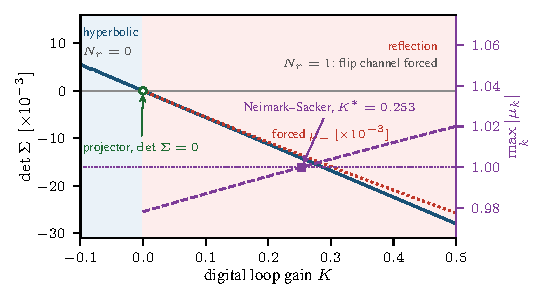
\includegraphics[width=\columnwidth]{figs/retardo_digital.pdf}
\caption{Digital control delay. The sample-and-hold is a rank-one factor
\eqref{eq:muestreador} whose type the loop gain selects: hyperbolic for
$K<0$, an exact projector at $K=0$, and reflection for every $K>0$, so
$N_r=1$ and a real negative multiplier (lower trace) is forced at
arbitrarily small positive gain. The orbit stays stable until $K^{*}=0.253$
and then loses stability through a complex pair; the forced negative
multiplier is still inside the unit circle when the pair crosses.}
\label{fig:fronteras}
\end{figure}

\subsection{Simultaneous Events and the Separation Hypothesis}
\label{sec:esquina}
When two events coincide, the order of the corresponding factors in
\eqref{eq:monodromy} is not fixed by the dynamics. For given saltation
matrices the order does not affect $\det M$, since
$\det(S_aS_b)=\det(S_bS_a)$, but the saltations must be rebuilt in each
order. Without magnetic coupling the two saltations of parallel modules
commute and the corner is removable. With coupled inductors and unequal
phases ($L_2/L_1=1.6$, $k=0.5$), $\det M$ depends on the order, $5.505$
against $22.010$, and the true monodromy converges to a different candidate
from each side of the corner \cite{dibernardo2001corner,burden2016}. In a
randomized search over $3000$ coupled pairs, one of the $1029$ admissible
corners has an order-dependent $N_r$, and it lies next to the singular type
boundary of Proposition~\ref{prop:species}. Both orders are transversal, and
\eqref{eq:parity} returns the correct sign for each. The count $N_r$ is
therefore not defined at a coupled simultaneous corner, and
Proposition~\ref{prop:parity} carries the separation hypothesis for this
reason. The plant, the search and the lateral limits of $\det M$ are
reported in Section~S-VI of the supplementary material.

\section{Discussion and Limitations}
\label{sec:discussion}
The lift is not proposed as a faster numerical method. Stored as the list of
its vector factors, the versor of a cycle costs a constant factor of about
ten over the matrix product (Section~\ref{sec:campana}), and by
\eqref{eq:grades} its scalars can equally be evaluated from $n\times n$
determinants. What the lift provides is a structural description of the
switched dynamics. Each nonsingular saltation
has a lift whose spinor norm is its determinant; that norm fixes the type
of the event and its contribution to the parity and to the volume budget,
and the grades of the total lift give the remaining coefficients of the
characteristic polynomial. The algebra supplies the identification of the
types and the closed forms, and it complements the border-collision program
\cite{ghosh2025robust,simpson2025zero,fatoyinbo2023synopsis} by computing
determinant signs and traces from the switched flow that generates the map,
where normal-form studies take them as parameters. In the coordinates of the stored energy, the interval flows of the
platform of Section~\ref{sec:ramp} differ from Euclidean rotations by less
than $3\%$. A rotation does not contribute to
\eqref{eq:budget}, and the budget therefore adds up the non-rigid part of
the cycle, namely the dissipation of the intervals and the factor
$\lvert1+\sigma_k\rvert$ of each event.

The results can be applied without computing eigenvalues. At an operating
point, the crossing-velocity ratio $\dot h^{+}/\dot h^{-}$ gives the type
of each event; in peak-current control the ramp slope $m_a=m_2$ separates
reflection from pass-through through the singular case. Under the hypotheses
of Proposition~\ref{prop:parity}, an odd reflection count guarantees a real
negative multiplier and, in a second-order converter, excludes a
complex-pair instability. In a two-phase converter, the comparison of
$\lvert\Delta\mu\rvert$ with $2\chi$ indicates whether the subharmonic
appears with a slow modulation (Section~\ref{sec:par}).

Two limitations are now delimited. Sample-and-hold control enters through
one more rank-one factor \eqref{eq:muestreador}, so a delayed digital loop
keeps the same types and the same count. Simultaneous events require
separate treatment: the corner is removable when the switching functions
are decoupled, and with coupling the derivative of the cycle map depends on
the order of the events; next to a type boundary $N_r$ itself can cease
to be a property of the operating point (Section~\ref{sec:esquina}). The
budget remains exact on each branch. No hardware was built for this paper.
The evidence beyond our own simulations consists of the published
multipliers of Table~\ref{tab:literatura} and of the published multipliers
and experimental waveforms of the voltage-mode buck converter
(Section~\ref{sec:otros}). Further work includes the invariant decomposition
\cite{roelfs2023graded} of the orientation-preserving part of $\bm{W}$ for
higher-order converters, the extension of the interference criterion of
Section~\ref{sec:par} to more than two phases and to coupled inductors, the
homogeneous extension
to $\mathcal{G}(n+1,n+1)$, which would include the source terms and the
periodic orbit in the same versor, and verification with a physical
controller in the loop.

\section{Conclusion}
Floquet analysis of switched converters has an exact representation in
$\Gnn$. The lifted monodromy is an ordered geometric product, and each
saltation lifts to $1+\bm{u}\bm{n}$, whose spinor norm equals its
determinant. The sign of that norm distinguishes the three event types,
and the rapidity describes the contraction of each event. Under the stated
event hypotheses, odd reflection parity forces a real negative multiplier;
among state-triggered switchings with continuous state, only a latched one
can reverse orientation. The lift carries the characteristic polynomial, so
flip and fold boundaries are zeros of scalars, and three scalars give a
complete stability test for second-order converters. For two phases, the
interference between the two reflections provides a closed-form threshold on
the mismatch, which separates a torus from a period doubling and agrees with
time-domain simulation. Simulations of buck, boost and interleaved converters with
conduction losses, ESR, diode models and component tolerances confirmed the
predicted multipliers by independent identification to better than
$10^{-4}$, and the gap between the exact subharmonic boundary and the
classical ramp rule has a closed form. Published multipliers for boost,
interleaved, photovoltaic and resonant converters are consistent with the
parity rule, those of the voltage-mode buck converter are reproduced to the
digits printed, and the hybrid-DAE example identifies the covector as the
quantity the algebra transports.

\section*{Reproducibility}
Python scripts (\texttt{clifford}, \texttt{scipy}) that reproduce every
figure and table, check Propositions~\ref{prop:species} and
\ref{prop:grades} for generic $\bm{u}_k$, $\bm{n}_k$ in
$\mathcal{G}(2,2)$--$\mathcal{G}(4,4)$, and recompute the running example
\eqref{eq:ejemplo} from the circuit model are provided as supplementary
material and at
\texttt{github.com/paketecuen/\allowbreak{}geometric-floquet-converters}.
The comparison of versor representations of Section~\ref{sec:campana}
additionally requires the library of \cite{eid2025gafl}.

\section*{Acknowledgment}
The authors thank Dr.~A.~H.~Eid for providing the numerical library used in
Section~\ref{sec:campana}.

\begin{thebibliography}{44}

\bibitem{deane1990instability} J. H. B. Deane and D. C. Hamill,
``Instability, subharmonics, and chaos in power electronic systems,''
\emph{IEEE Trans. Power Electron.}, vol. 5, no. 3, pp. 260--268, Jul. 1990,
doi: 10.1109/63.56516.

\bibitem{banerjee2001nonlinear} S. Banerjee and G. C. Verghese, Eds.,
\emph{Nonlinear Phenomena in Power Electronics: Attractors, Bifurcations,
Chaos, and Nonlinear Control}. New York, NY, USA: Wiley-IEEE Press, 2001.

\bibitem{aizerman1958} M. A. Aizerman and F. R. Gantmakher, ``On the
stability of periodic motions,'' \emph{J. Appl. Math. Mech.}, vol. 22,
no. 6, pp. 1065--1078, 1958, doi: 10.1016/0021-8928(58)90033-9.

\bibitem{muller1995} P. C. M\"uller, ``Calculation of Lyapunov exponents for
dynamic systems with discontinuities,'' \emph{Chaos Solitons Fractals},
vol. 5, no. 9, pp. 1671--1681, Sep. 1995.

\bibitem{leine2004} R. I. Leine and H. Nijmeijer, \emph{Dynamics and
Bifurcations of Non-Smooth Mechanical Systems}. Berlin, Germany: Springer, 2004.

\bibitem{kong2024saltation} N. J. Kong, J. J. Payne, J. Zhu, and
A. M. Johnson, ``Saltation matrices: The essential tool for linearizing
hybrid dynamical systems,'' \emph{Proc. IEEE}, vol. 112, no. 6,
pp. 585--608, Jun. 2024, doi: 10.1109/JPROC.2024.3440211.

\bibitem{giaouris2008stability} D. Giaouris, S. Banerjee, B. Zahawi, and
V. Pickert, ``Stability analysis of the continuous-conduction-mode buck
converter via Filippov's method,'' \emph{IEEE Trans. Circuits Syst. I,
Reg. Papers}, vol. 55, no. 4, pp. 1084--1096, May 2008.

\bibitem{elaroudi2015review} A. El Aroudi, D. Giaouris, H. H.-C. Iu, and
I. A. Hiskens, ``A review on stability analysis methods for switching mode
power converters,'' \emph{IEEE J. Emerg. Sel. Topics Circuits Syst.},
vol. 5, no. 3, pp. 302--315, Sep. 2015.

\bibitem{elaroudi2021analytical} A. El Aroudi, M. S. Al-Numay, R. Haroun,
and G. Zhang, ``Analytical determination of fast-scale instability
boundaries for current mode controlled DC--DC converters with CPL and closed
voltage loop,'' \emph{IEEE J. Emerg. Sel. Topics Circuits Syst.}, vol. 11,
no. 1, pp. 39--48, Mar. 2021, doi: 10.1109/JETCAS.2021.3052861.

\bibitem{erickson2020fundamentals} R. W. Erickson and D. Maksimovi\'c,
\emph{Fundamentals of Power Electronics}, 3rd ed. Cham, Switzerland:
Springer, 2020.

\bibitem{elaroudi2020piecewise} A. El Aroudi, K. Mandal, M. S. Al-Numay,
D. Giaouris, and S. Banerjee, ``Piecewise quadratic slope compensation
technique for DC--DC switching converters,'' \emph{IEEE Trans. Circuits
Syst. I, Reg. Papers}, vol. 67, no. 12, pp. 5574--5585, Dec. 2020, doi:
10.1109/TCSI.2020.2993793.

\bibitem{mandal2013symmetry} K. Mandal, S. Banerjee, and C. Chakraborty,
``Symmetry-breaking bifurcation in series-parallel load resonant DC--DC
converters,'' \emph{IEEE Trans. Circuits Syst. I, Reg. Papers}, vol. 60,
no. 3, pp. 778--787, Mar. 2013.

\bibitem{wu2014interleaved} H. Wu, V. Pickert, and D. Giaouris,
``Nonlinear analysis for interleaved boost converters based on monodromy
matrix,'' in \emph{Proc. IEEE Energy Convers. Congr. Expo. (ECCE)},
Pittsburgh, PA, USA, Sep. 2014, pp. 2511--2516.

\bibitem{giaouris2009filippov} D. Giaouris, S. Maity, S. Banerjee,
V. Pickert, and B. Zahawi, ``Application of Filippov method for the analysis
of subharmonic instability in dc--dc converters,'' \emph{Int. J. Circuit
Theory Appl.}, vol. 37, no. 8, pp. 899--919, Oct. 2009.

\bibitem{doran1993lie} C. Doran, D. Hestenes, F. Sommen, and N. Van Acker,
``Lie groups as spin groups,'' \emph{J. Math. Phys.}, vol. 34, no. 8,
pp. 3642--3669, Aug. 1993.

\bibitem{lounesto2001} P. Lounesto, \emph{Clifford Algebras and Spinors},
2nd ed. Cambridge, U.K.:
Cambridge Univ. Press, 2001.

\bibitem{kuznetsov2004} Y. A. Kuznetsov, \emph{Elements of Applied
Bifurcation Theory}, 3rd ed. New York, NY, USA: Springer, 2004.

\bibitem{horn2013matrix} R. A. Horn and C. R. Johnson, \emph{Matrix
Analysis}, 2nd ed. Cambridge, U.K.: Cambridge Univ. Press, 2013.

\bibitem{montoya_gapot1} F. G. Montoya, R. Ba\~nos, A. Alcayde,
F. M. Arrabal-Campos, and J. Rold\'an-P\'erez, ``Vector geometric algebra in
power systems: An updated formulation of apparent power under non-sinusoidal
conditions,'' \emph{Mathematics}, vol. 9, no. 11, art. no. 1295, Jun. 2021.

\bibitem{montoya_gapot3} F. G. Montoya and A. H. Eid, ``Formulating the
geometric foundation of Clarke, Park, and FBD transformations by means of
Clifford's geometric algebra,'' \emph{Math. Methods Appl. Sci.}, vol. 45,
no. 8, pp. 4252--4277, May 2022.

\bibitem{velasco2025introducing} M. Velasco, I. Zaplana, A. D\`oria-Cerezo,
J. Duarte, and P. Mart\'i, ``Introducing modeling, analysis, and control of
three-phase electrical systems using geometric algebra,'' \emph{IEEE Trans.
Ind. Electron.}, vol. 72, no. 11, pp. 10906--10915, Nov. 2025, doi:
10.1109/TIE.2025.3553169.

\bibitem{sira2022lyapunov} H. Sira-Ram\'irez, B. C. G\'omez-Le\'on, and
M. A. Aguilar-Ordu\~na, ``Lyapunov stability: A geometric algebra
approach,'' \emph{Adv. Appl. Clifford Algebras}, vol. 32, no. 2,
art. no. 26, 2022.

\bibitem{sira2023sliding} H. Sira-Ram\'irez, M. A. Aguilar-Ordu\~na, and
B. C. G\'omez-Le\'on, ``Sliding mode control of switched systems: A
geometric algebra approach,'' \emph{Asian J. Control}, vol. 25, no. 1,
pp. 15--25, Jan. 2023.

\bibitem{sira2023invariance} H. Sira-Ram\'irez, B. C. G\'omez-Le\'on, and
M. A. Aguilar-Ordu\~na, ``A geometric algebra approach to invariance control
in sliding regimes for switched systems,'' \emph{Adv. Appl. Clifford
Algebras}, vol. 33, no. 3, art. no. 35, 2023.

\bibitem{sira2025hamiltonian} H. Sira-Ram\'irez, B. C. G\'omez-Le\'on, and
M. A. Aguilar-Ordu\~na, ``Sliding mode control of switched Hamiltonian
systems: A geometric algebra approach,'' \emph{Adv. Appl. Clifford
Algebras}, vol. 35, no. 2, art. no. 19, 2025.

\bibitem{derevianko2024solverfree} A. Derevianko and P. Va\v{s}\'ik,
``Solver-free optimal control for linear dynamical switched system by means
of geometric algebra,'' \emph{Math. Methods Appl. Sci.}, vol. 47, no. 3,
pp. 1274--1288, 2024.

\bibitem{ghosh2025robust} I. Ghosh, R. I. McLachlan, and D. J. W. Simpson,
``Robust chaos in orientation-reversing and noninvertible two-dimensional
piecewise-linear maps,'' \emph{J. Nonlinear Sci.}, vol. 35, no. 1,
art. no. 16, 2025.

\bibitem{simpson2025zero} D. J. W. Simpson, ``The two-dimensional
border-collision normal form with a zero determinant,'' \emph{SIAM J.
Appl. Dyn. Syst.}, vol. 24, no. 3, pp. 2205--2245, 2025.

\bibitem{fatoyinbo2023synopsis} H. O. Fatoyinbo and D. J. W. Simpson,
``A synopsis of the noninvertible, two-dimensional, border-collision normal
form with applications to power converters,'' \emph{Int. J. Bifurcation
Chaos}, vol. 33, no. 8, art. no. 2330019, 2023,
doi: 10.1142/S0218127423300197.

\bibitem{parui2002border} S. Parui and S. Banerjee, ``Border collision
bifurcations at the change of state-space dimension,'' \emph{Chaos}, vol. 12, no. 4,
pp. 1054--1069, Dec. 2002.

\bibitem{swift1984suppression} J. W. Swift and K. Wiesenfeld,
``Suppression of period doubling in symmetric systems,'' \emph{Phys. Rev.
Lett.}, vol. 52, no. 9, pp. 705--708, Feb. 1984.

\bibitem{hayes2020application} B. Hayes, M. Condon, and D. Giaouris,
``Application of the Filippov method to PV-fed DC--DC converters modeled as
hybrid-DAEs,'' \emph{Eng. Rep.}, vol. 2, no. 9, p. e12237, Sep. 2020,
doi: 10.1002/eng2.12237.

\bibitem{dibernardo2008} M. di Bernardo, C. J. Budd, A. R. Champneys, and
P. Kowalczyk, \emph{Piecewise-smooth Dynamical Systems: Theory and
Applications}. London, U.K.:
Springer, 2008.

\bibitem{filippov1988} A. F. Filippov, \emph{Differential Equations with
Discontinuous Righthand Sides}. Dordrecht, The Netherlands: Kluwer, 1988.

\bibitem{ridley1991new} R. B. Ridley, ``A new, continuous-time model for
current-mode control,'' \emph{IEEE Trans. Power Electron.}, vol. 6, no. 2,
pp. 271--280, Apr. 1991, doi: 10.1109/63.76813.

\bibitem{iu2001bifurcation} H. H. C. Iu and C. K. Tse, ``Bifurcation
behavior in parallel-connected buck converters,'' \emph{IEEE Trans. Circuits
Syst. I: Fundam. Theory Appl.}, vol. 48, no. 2, pp. 233--240, Feb. 2001,
doi: 10.1109/81.904890.

\bibitem{giaouris2013foldings} D. Giaouris, S. Banerjee, F. Stergiopoulos,
S. Papadopoulou, S. Voutetakis, B. Zahawi, V. Pickert, A. Abusorrah,
M. Al Hindawi, and Y. Al-Turki, ``Foldings and grazings of tori in current
controlled interleaved boost converters,'' \emph{Int. J. Circuit Theory
Appl.}, vol. 42, no. 10, pp. 1080--1091, Oct. 2014, doi: 10.1002/cta.1906.

\bibitem{fossas1996study} E. Fossas and G. Olivar, ``Study of chaos in the
buck converter,'' \emph{IEEE Trans. Circuits Syst. I: Fundam. Theory Appl.},
vol. 43, no. 1, pp. 13--25, Jan. 1996, doi: 10.1109/81.481457.

\bibitem{eid2025gafl} A. H. Eid, ``GeometricAlgebraFulcrumLib: A unified
generic C\# library for geometric algebra computations,'' GitHub repository,
2025. [Online]. Available:
\texttt{https://github.com/\allowbreak{}ga-explorer/\allowbreak{}GeometricAlgebraFulcrumLib}

\bibitem{middlebrook1976} R. D. Middlebrook, ``Input filter considerations
in design and application of switching regulators,'' in \emph{Proc. IEEE
Ind. Appl. Soc. Annu. Meeting}, Chicago, IL, USA, Oct. 1976, pp. 366--382.

\bibitem{dranga2003stability} O. Dranga, B. Buti, and I. Nagy, ``Stability
analysis of a feedback-controlled resonant DC--DC converter,'' \emph{IEEE
Trans. Ind. Electron.}, vol. 50, no. 1, pp. 141--152, Feb. 2003,
doi: 10.1109/TIE.2002.804983.

\bibitem{imrayed2013controlling} O. Imrayed, I. Daho, and H. M. Amreiz,
``Controlling nonlinear behavior in current mode controlled boost converter
based on the monodromy matrix,'' \emph{Conf. Papers Eng.}, vol. 2013,
pp. 1--7, 2013, doi: 10.1155/2013/683421.

\bibitem{liu2025filippov} Z. Liu, M. Su, J. Lin, Y. Sun, H. Li, X. Li, and
Y. Liu, ``Filippov-based stability analysis of digitally controlled
single-phase grid-tied inverter,'' \emph{IEEE Trans. Ind. Electron.},
vol. 72, no. 10, pp. 10028--10039, Oct. 2025, doi: 10.1109/TIE.2025.3552264.

\bibitem{dibernardo2001corner} M. di Bernardo, C. J. Budd, and
A. R. Champneys, ``Corner collision implies border-collision bifurcation,''
\emph{Physica D}, vol. 154, no. 3--4, pp. 171--194, Jun. 2001,
doi: 10.1016/S0167-2789(01)00250-0.

\bibitem{burden2016} S. A. Burden, S. S. Sastry, D. E. Koditschek, and
S. Revzen, ``Event-selected vector field discontinuities yield
piecewise-differentiable flows,'' \emph{SIAM J. Appl. Dyn. Syst.}, vol. 15,
no. 2, pp. 1227--1267, 2016, doi: 10.1137/15M1016588.

\bibitem{roelfs2023graded} M. Roelfs and S. De Keninck, ``Graded symmetry
groups: Plane and simple,'' \emph{Adv. Appl. Clifford Algebras}, vol. 33,
no. 3, art. no. 30, 2023.

\end{thebibliography}

\end{document}
